%%
%% This is file `mitsample.tex',
%% generated with the docstrip utility.
%
% The original source files were:
%
% ubcthesis.dtx  (with options: `mitsampletex')
%% 
%% This file was generated from the ubcthesis package.
%% --------------------------------------------------------------
%% 
%% Copyright (C) 2001
%% Michael McNeil Forbes
%% mforbes@alum.mit.edu
%% 
%% This file may be distributed and/or modified under the
%% conditions of the LaTeX Project Public License, either version 1.2
%% of this license or (at your option) any later version.
%% The latest version of this license is in
%%    http://www.latex-project.org/lppl.txt
%% and version 1.2 or later is part of all distributions of LaTeX
%% version 1999/12/01 or later.
%% 
%% This program is distributed in the hope that it will be useful,
%% but WITHOUT ANY WARRANTY; without even the implied warranty of
%% MERCHANTABILITY or FITNESS FOR A PARTICULAR PURPOSE.  See the
%% LaTeX Project Public License for more details.
%% 
%% This program consists of the files ubcthesis.dtx, ubcthesis.ins, and
%% the sample figures fig.eps and fig.fig.
%% 
%% This file may be modified and used as a base for your thesis without
%% including the licence agreement as long as the content (i.e. textual
%% body) of the file is completely rewritten. You must, however, change
%% the name of the file.
%% 
%% This file may only be distributed together with a copy of this
%% program. You may, however, distribute this program without generated
%% files such as this one.
%% 


% This Sample thesis requires \LaTeX2e
\NeedsTeXFormat{LaTeX2e}[1995/12/01]
\ProvidesFile{mitsample.tex}[2006/09/02 v1.42 ^^J
 Massachusetts Institute of Technology Sample Thesis]

\documentclass[msc,12pt,upper,appendixpart,appendixpage,oneside,logo,bold,norunningheaders,tocupper,tocitalic,a4paper]{mitthesis}
\usepackage[T1]{fontenc}
\usepackage[spanish]{babel} 
\usepackage{ucs}
\usepackage[utf8]{inputenc}
\usepackage[spanish]{babel}
\usepackage{setspace}
\usepackage{ulem}
\usepackage{longtable}
%
% To compile issue the following commands:
% latex mitsample
% bibtex mitsample
% latex mitsample
% latex mitsample
% latex mitsample
%
% To view use xdvi (on unix systems):
% xdvi mitsample.dvi
%
% To make a postscript file, use dvips:
% dvips -o mitsample.ps mitsample.dvi
%
% To view the postscript file, use ghostview or gv (on unix systems):
% gv mitsample.ps
%
%************************************************
% Optional packages.
%
% The use of these packages is optional: they are standard now and
% should be installed on your system, but if they are not, you might
% have to comment out the appropriate lines to get this file to
% compile.
%
%******** natbib ********************************
% This is a very nice package for bibliographies.  It includes options
% for sorting and compressing bibliographic entries.
\usepackage[numbers,sort&compress]{natbib}

%******** graphics and graphicx ******************************
% This allows you to include encapsulated postscript files.  If you
% don't have this, comment the \includegraphics{} line following the
% comment "%includegraphics" later in this file.
\usepackage[dvips]{graphicx}
\DeclareGraphicsRule{.emf}{bmp}{}{}
\DeclareGraphicsExtensions{.pdf,.png,.jpg} %solo para PDFLaTeX

%******** lscape ******************************
% This allows you to include landscape layout pages by using the
% |landscape| environment. Note that this output might only be valid
% after converting to a postscript or pdf file.
\usepackage{lscape}

%******** psfrag ******************************
% This allows you to replace text in postscript pictures with formated
% latex text.  This allows you to use math in graph labels
% etc. Uncomment the psfrag lines following the "%psfrag" comment
% later in this file if you don't have this package.  The replacements
% will only be visible in the final postscript file: they will be
% listed in the .dvi file but not performed.
\usepackage{psfrag}

%******** afterpage ***************************
% This package allows you to issue commands at the end of the current
% page.  A good use for this is to use the command
% \afterpage{\clearpage} right after a figure.  This will cause the
% figure to be inserted on the page following the current one (or on
% the current page if it will fit) but will not break the page in the
% middle.
\usepackage{afterpage}

%******** hyperref *****************************
% This adds hyperlinks to your document: with the right viewers (later
% versions of xdvi, acrobat with pdftex, latex2html etc.) this will
% make your equation, figure, citation references etc. hyperlinks so
% that you can click on them.  Also, your table of contents will be
% able to take you to the appropriate sections.  In the viewers that
% support this, the links often appear with an underscore.  This
% underscore will not appear in printed versions.
%
% Note: if you do not use the hypertex option, then the dvips driver
% may be loaded by default.  This will cause the entries in the list
% of figures and list of tables to be on a single line because dvips
% does not deal with hyperlinks on broken lines properly.
%
% Also, the hyperref package should be loaded last as it modified the
% commands in many other pagckages.
\usepackage[hypertex]{hyperref}
\usepackage{fancyhdr}
\usepackage{url}
% If you would like to compile this sample thesis without the
% hyperref package, then you will need to comment out the previous
% \usepackage command and uncomment the following command which will
% put the URL's in a typewriter font but not link them.
%\newcommand\href[2]{\texttt{#2}}
%\renewcommand*\familydefault{\sfdefault}
\renewcommand{\rmdefault}{phv} % Arial
\renewcommand{\sfdefault}{phv} % Arial

% These commands are optional.  The defaults are shown.
\institution{Escuela Superior Polit\'ecnica del Litoral}
\institutionaddress{Guayaquil, Ecuador}
\program{Maestr\'ia en Sistemas de Informaci\'on Gerencial}
\gracias{A Dios, \\a mis padres y \\a mis profesores}
\dedicado{Con cari\~no,\\ para mis padres}
% You can issue as many of these as you have...
%\previousdegree{B.Sc., The University of British Columbia, 1999}
%\previousdegree{M.Sc., The University of British Columbia, 2001}

% You can override the option setting here.
 \degreetitle{Ingeniero en Computaci\'on especializaci\'on Sistemas Multimedia}

% These commands are required.
\title{``IMPLEMENTACI\'ON DEL PORTAL WEB DE ADMINISTRACI\'ON DE EVENTOS PARA GRUPOS DE INVESTIGACI\'ON''}
\author{Guillermo Omar Pizarro V\'asquez \\ Rafael Eduardo Rivadeneira Campodonico}
\copyrightyear{2009}
\submitdate{\today}

% These commands are required by MIT.
\advisor{Ing. M\'onica Villavicencio}
\departmentchair{Ing. Jorge Aragundi}
\mtribunalp{M.Sc. }
\mtribunals{M.Sc. }
% One might want to override the format of the section and chapter3
% numbers.  This shows you how to do it.  Note that
\renewcommand\thepart         {\Roman{part}}
\renewcommand\thechapter      {\Roman{chapter}}
\renewcommand\thesection      {}
\renewcommand\thesubsection   {}
\renewcommand\thesubsubsection{\thesubsection.\arabic{subsubsection}}
\renewcommand\theparagraph    {\thesubsubsection.\arabic{paragraph}}
\renewcommand\thesubparagraph {\theparagraph.\arabic{subparagraph}}

\setcounter{tocdepth}{2}
\setlength{\parindent}{0pt}

% Here is the start of the document.
\begin{document}

% Unlike the UBC thesis, page numbering for MIT theses should start
% at 1 and continue.  Thus, there is no \frontmatter command issued
% here as there was for the UBC thesis.
\maketitle
\frontmatter
\agradecimiento
\dedicatoria
\tribunal
\authorizationform

\begin{abstract}
El presente Proyecto de Grado tiene el prop\'osito de implementar una Aplicaci\'on Web, utilizando conjuntamente las metodolog\'ias \textbf{MDA} (Model Driven Architecture) y \textbf{MERODE} (Model - driven, Existence - dependency Relation Object - oriented DEvelopment), para facilitar la Administraci\'on de un Evento en un Grupo de Investigaci\'on.

Es importante mencionar que anteriormente se ha implementado, como Proyecto de Tesis, un producto llamado AppVlir8\footnote{\url{http://www.vlir8.espol.edu.ec}}, el mismo que es tambi\'en un Portal Web de Administraci\'on de eventos. Nuestra idea es retomar el dise\~no original de este software y modificarlo, corrigiendo defectos y agregando mejoras cuya necesidad se ha identificado durante el tiempo en que el software ha estado en producci\'on (a partir de Septiembre del 2006).

En el primer cap\'itulo se se\~nalan los antecedentes de retomar este Proyecto, el hecho de que MERODE si ayuda en el dise\~no independiente del dominio, vital para seguir la metodolog\'ia MDA, aunque se va a usar la misma tecnolog\'ia J2EE, utilizada en AppVlir8, pero con la especificaci\'on JSP 2.0 siguiendo el patr\'on de dise\~no MVC 2, los objetivos que se espera alcanzar y la justificaci\'on del desarrollo de los m\'odulos.

En el segundo cap\'itulo se redactan los fundamentos te\'oricos en los que se basa este Proyecto de Grado, justificando el uso de cada elemento incluido en la arquitectura del mismo.

En el tercer cap\'itulo se documentan los requerimientos funcionales y no funcionales levantados para mejorar el dise\~no del anterior Sistema. Adem\'as de la especificaci\'on del PIM y del PSM, previos a la fase de la transformaci\'on al c\'odigo.

En el cuarto cap\'itulo se mencionan los cambios realizados en la Arquitectura del Sistema anterior y las novedades en el actual, para poder satisfacer algunos requerimientos claves del usuario del Sistema.

En el quinto cap\'itulo se realiza un an\'alisis con respecto a la implementaci\'on realizada y las pruebas que se realizaron para la entrega de un producto de calidad.

Finalmente se exponen las conclusiones y recomendaciones del Proyecto de Grado.
\end{abstract}


\tableofcontents
\listoffigures
\listoftables
\addtocontents{toc}{\vspace*{\baselineskip}}
\newpage

% Any other unusual sections should come here between the
% acknowledgements and the main body.
\mainmatter
% Suppress the running headers for this page only.
\thispagestyle{plain}

\fancypagestyle{plain}{%
\fancyhf{}
\renewcommand{\headrulewidth}{0pt}}
\setlength{\parskip}{\baselineskip}
 
% Here we provide a short optional argument to \chapter[]{}.  This
% optional argument will appear in the table of contents.  For long
% titles, one should use this to give a single-line entry to the
% table of contents.

\chapter{Antecedentes}
\begin{indentar}
\end{indentar}

\section{Antecedentes}
\begin{indentar}
\end{indentar}

\section{Justificaci\'on}
\begin{indentar}
\end{indentar}

\section{Objetivos}
\begin{indentar}
\end{indentar}
\chapter{Fundamentos Te\'oricos}
\begin{indentar}
\end{indentar}

\section{Descripci\'on General de MDA y MERODE}
\begin{indentar}
\end{indentar}

\section{Tecnolog\'ias Open Source}
\begin{indentar}
\end{indentar}

\subsection{Uso de la arquitectura J2EE.}
\begin{indentar}
\end{indentar}

\subsection{Librer\'ias en el Servidor: JSTL, JSON y Velocity.}
\begin{indentar}
\end{indentar}

\subsection{Librer\'ias en el Cliente: Dojo y YUI.}
\begin{indentar}
\end{indentar}

\subsection{Base de Datos: MySQL y HSQLDB.}
\begin{indentar}
\end{indentar}

\subsection{Uso de la herramienta CASE: StarUML.}
\begin{indentar}
\end{indentar}
\chapter{An\'alisis del Sistema}
\section{Requerimientos Funcionales}
\begin{indentar}
De manera general, los requerimientos que se han pedido para mejorar el Portal son los siguientes:
\begin{itemize}
\item A\~nadir el m\'odulo de pago en l\'inea;
\item Dar soporte para varios idiomas;
\item Mostrar res\'umenes de evaluaciones, con los siguientes datos: recomendaci\'on y exportaci\'on de los datos ingresados por los evaluadores;
\item Implementar requerimientos adicionales pedidos por el Sub - Componente de Telecomunicaciones, tales como:
	\begin{itemize}
	\item Manejar copias ocultas para emails de rechazo de art\'iculos, es decir, el correo electr\'onico debe enviarse con copia al correo electr\'onico del evento y con copia oculta al administrador que rechaza el art\'iculo;
	\item Mayor flexibilidad en el momento de la elaboraci\'on y modificaci\'on de las preguntas frecuentes;
	\item Agregar la posibilidad de subir un resumen previo -por parte del usuario participante del evento cient\'ifico- al art\'iculo cient\'ifico final  que se va a evaluar;
	\item Se debe poder modificar un art\'iculo sin tener que borrar y volverlo a subir;
	\item Despu\'es de evaluado un art\'iculo, se debe seguir mostrando -a los administradores del evento- quienes fueron sus evaluadores;
	\item El registro del usuario debe ser internacional y no s\'olo dirigido a nuestro pa\'is;
	\item Corregir lo siguiente: un autor no debe poder evaluar su propio art\'iculo, los autores secundarios tambi\'en deben constar en la lista de un art\'iculo, y en el manejo de sesiones (a veces se sale del sistema y se desea ingresar con clave err\'onea, el sistema lo permite);
	\item Generar los siguientes reportes: trabajos por autores, evaluadores asignados a cada art\'iculo, res\'umenes de art\'iculos clasificados con su respectiva nota y el estado de cada art\'iculo. Exportar los reportes a los formatos: CSV y pdf;
	\item Adjuntar los art\'iculos de derecho de traspaso de los art\'iculos aceptados;
	\item Permitir que el administrador pueda eliminar un art\'iculo;
	\item Ocultar clave de la lista de los usuarios;
	\item Manejar un email de contacto para cada evento diferente;
	\item Guardar la fecha de publicaci\'on de un art\'iculo, cuando se lo suba al Sistema;
	\item En los registros: cuando un usuario realice un pago en efectivo, permitir ingresar el valor que pag\'o; en el pre registro notificar al usuario la fecha l\'imite para realizar el pago correspondiente;
	\item Poder escoger el autor de un paper en caso de que una persona alterna suba el art\'iculo por el autor.
	\end{itemize}
\end{itemize}
\end{indentar}

\section{Requerimientos No Funcionales}
Los requerimientos no funcionales que se desea para el Portal son los siguientes:
\begin{indentar}
\begin{itemize}
\item Manejo m\'as apropiado de IHM\footnote{Interacci\'on Hombre - M\'aquina.}: estandarizaci\'on de los \'iconos de la aplicaci\'on y mostrar errores espec\'ificos, no generales. (Mejor retroalimentaci\'on);
\item Utilizar MVC 2 en el dise\~no e implementaci\'on; puesto que este ofrece mayor flexibilidad al producto final;
\item Reparar defectos encontrados, entre los cuales existen algunos que afectan al rendimiento de la Aplicaci\'on Web, tales como: la optimizaci\'on de las consultas a la Base de Datos;
\item Separar la parte de manejo de eventos para que pueda instalarse y ejecutarse independientemente de la parte de administraci\'on de grupos de investigaci\'on y sus \'areas de trabajo.
\end{itemize}
Los requerimientos m\'inimos, en cuanto a hardware, son los siguientes:
\begin{itemize}
\item Capacidad de memoria en el servidor: para un buen desempe\~no del sistema, una memoria de 2 GB de RAM \'o superior.
\item Capacidad de disco duro en el servidor: se recomienda un disco duro de 80 GB como m\'inimo.
\item Tipo de procesador en el servidor: Se recomienda un procesador Core 2 Duo 2.0GHz.
\item Ancho de Banda para el servidor: Ancho de Banda recomendado 128 Mbits.
\item Navegadores: Para un buen uso del sistema se recomienda Firefox 3.0 \'o superior.
\item Sistema Operativo en el Servidor: Microsoft Windows XP \'o superior, o cualquier distribuci\'on de GNU/Linux, se recomienda Ubuntu.
\end{itemize}
\end{indentar}

\section{Especificaci\'on del Modelo Independiente de la Plataforma (PIM) usando t\'ecnicas de MERODE}
\begin{indentar}
MERODE nos permite la posibilidad de modelar el dominio de manera independiente de la plataforma que se desee implementar en un futuro pr\'oximo, en nuestro caso deseamos diagramar un PIM (Platform Independent Model) mediante un EDG, fue dise\~nado mediante la herramienta llamada MERMAID\footnote{\url{http://merode.econ.kuleuven.ac.be/activate.aspx}}.

Es necesario mencionar, el hecho de haber diagramado en un solo PIM el dominio de la administraci\'on de usuarios, la administraci\'on de eventos, la convocatoria y la evaluaci\'on de art\'iculos. Al realizar esta actividad de revisi\'on y redise\~no, se ha pensado de manera sistem\'atica la diagramaci\'on de un solo PIM en varios m\'odulos.
\end{indentar}

\subsection{El gr\'afico de la dependencia de existencia (EDG)}
\begin{indentar}
A continuaci\'on se muestran los Gr\'aficos de la Dependencia de existencia o EDG, como sistema (\ref{edg:websae}) y luego separado por m\'odulos para un mejor estudio de ellos.

\begin{landscape}
\begin{figure}
  \centering
    {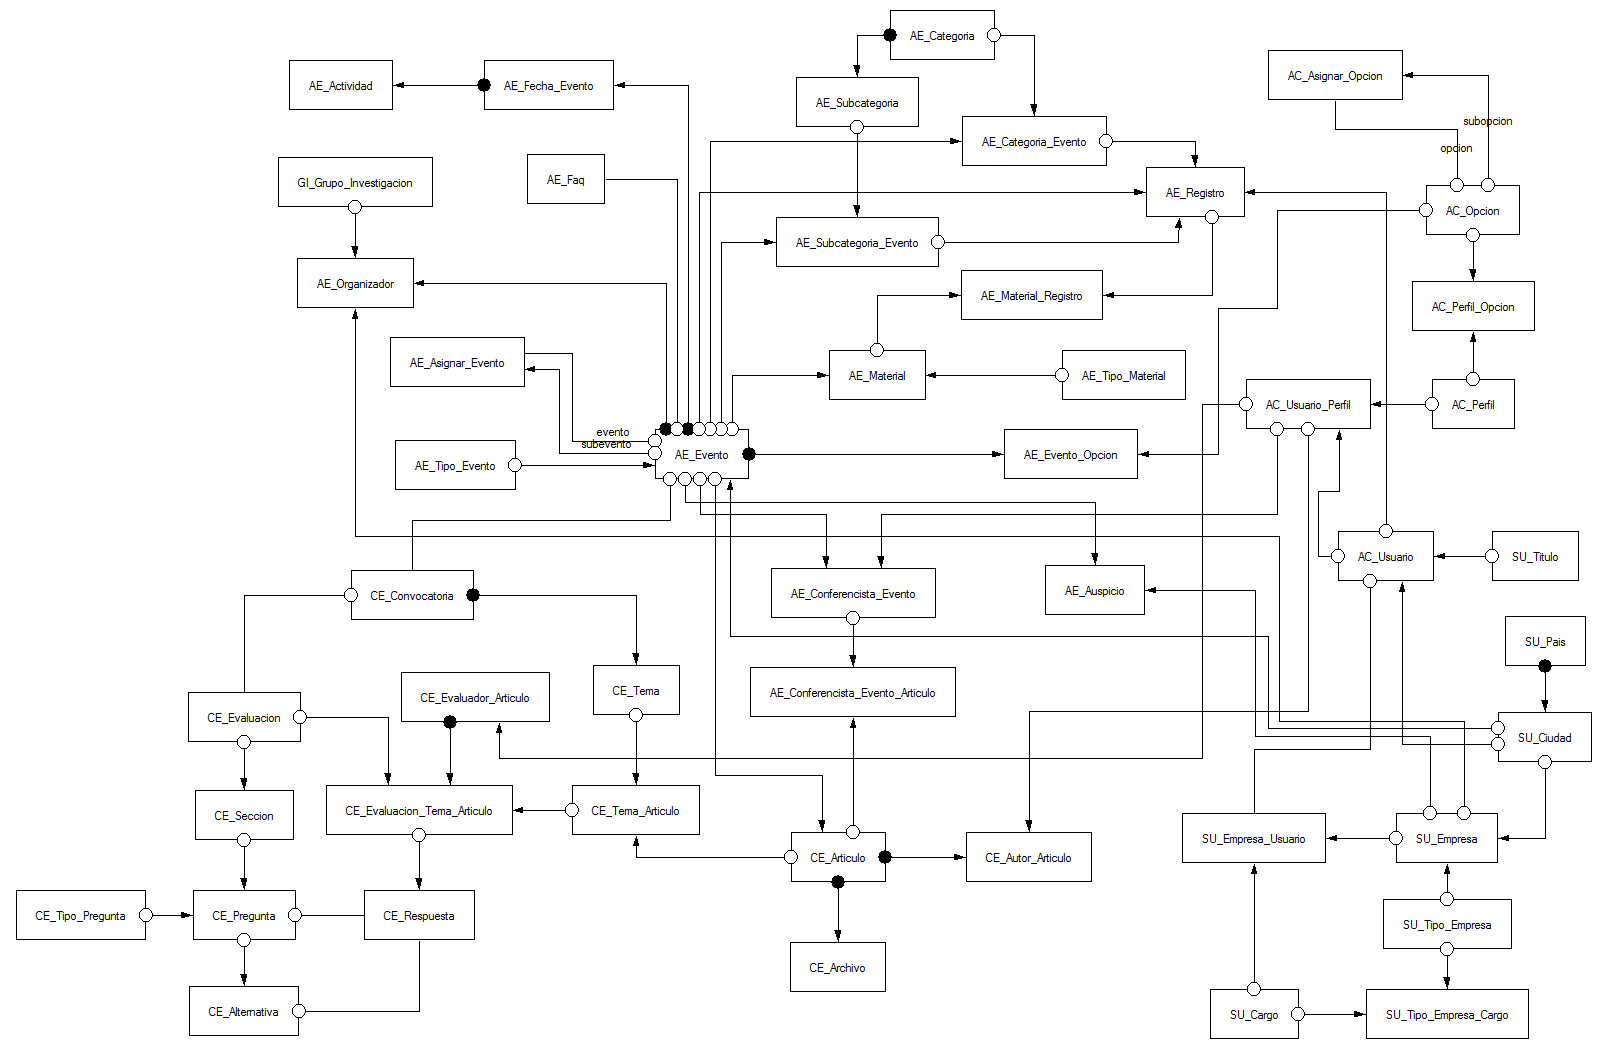
\includegraphics[width=1.5\textwidth]{images/merode-websae.eps}}
  \caption{EDG - Sistema Web para la Administraci\'on de Eventos Cient\'ificos (WebSAE)}
  \label{edg:websae}
\end{figure}
\end{landscape}

Se necesitaron un total de 48 objetos para implementar el Sistema actual, que ha sido denominado como \textbf{WebSAE}. En el Sistema original, denominado como \textbf{AppVlir8}, se dise\~n\'o con 42 objetos en total, es decir, que en el actual se han aumentado 6 objetos.

A continuaci\'on se enumerar\'an los objetos propios de cada m\'odulo con el correspondiente EDG:

\textbf{M\'ODULO DE ADMINISTRACI\'ON CENTRAL (MAC)}

\textbf{MAC} (\ref{edg:mac}) tiene 6 objetos que se listar\'an a continuaci\'on:

\begin{enumerate}
\item AC\_Usuario
\item AC\_Usuario\_Perfil
\item AC\_Perfil
\item AC\_Perfil\_Opcion
\item AC\_Opcion
\item AC\_Asignar\_Opcion
\end{enumerate}

Es necesario enfatizar que \textbf{MAC} surge en el momento de pensar en la Arquitectura de \textbf{WebSAE}, la mitad  de los objetos son nuevos, a continuaci\'on la siguiente ~\ref{diferencias:websae-appvlir8-mac} nos explica las diferencias entre los objetos, dependiendo si es el Sistema actual o el anterior.

\begin{table}
	\begin{center}
	\begin{tabular}{|p{1.5in}|p{1.5in}|p{1.8in}|}
		\hline
		\textbf{WebSAE} & \textbf{AppVlir8} & \textbf{Observaciones} \\
		\hline\hline
		  AC\_Usuario\_Perfil	& Rol\_Usuario &  \\
		\hline
		  AC\_Perfil				& Rol		 		&  \\
		\hline
		  AC\_Perfil\_Opcion		& Menu	 		& Objeto que asigna las opciones, dependiendo del perfil que se haya deseado crear. \\
		\hline
		  AC\_Opcion				& Opcion\_Menu	& Son las diversas opciones que se le presentan al usuario, dependiendo del perfil que tenga asignado.  \\
		\hline
		  AC\_Asignar\_Opcion	& Submenu 		& Este objeto nos sirve para manejar la recursi\'on entre las opciones, debido a que normalmente existen subopciones entre las opciones\footnote{\textbf{MERODE} no permite dise\~nar recursividad en un mismo objeto, por eso la necesidad de crear otro objeto que maneje este tipo de especificaciones.}. \\
		\hline
	\end{tabular}
	\caption{Diferencias entre los objetos de \textbf{WebSAE} y \textbf{AppVlir8}, en \textbf{MAC}.}\label{diferencias:websae-appvlir8-mac}
	\end{center}
\end{table}

\begin{figure}
  \centering
    {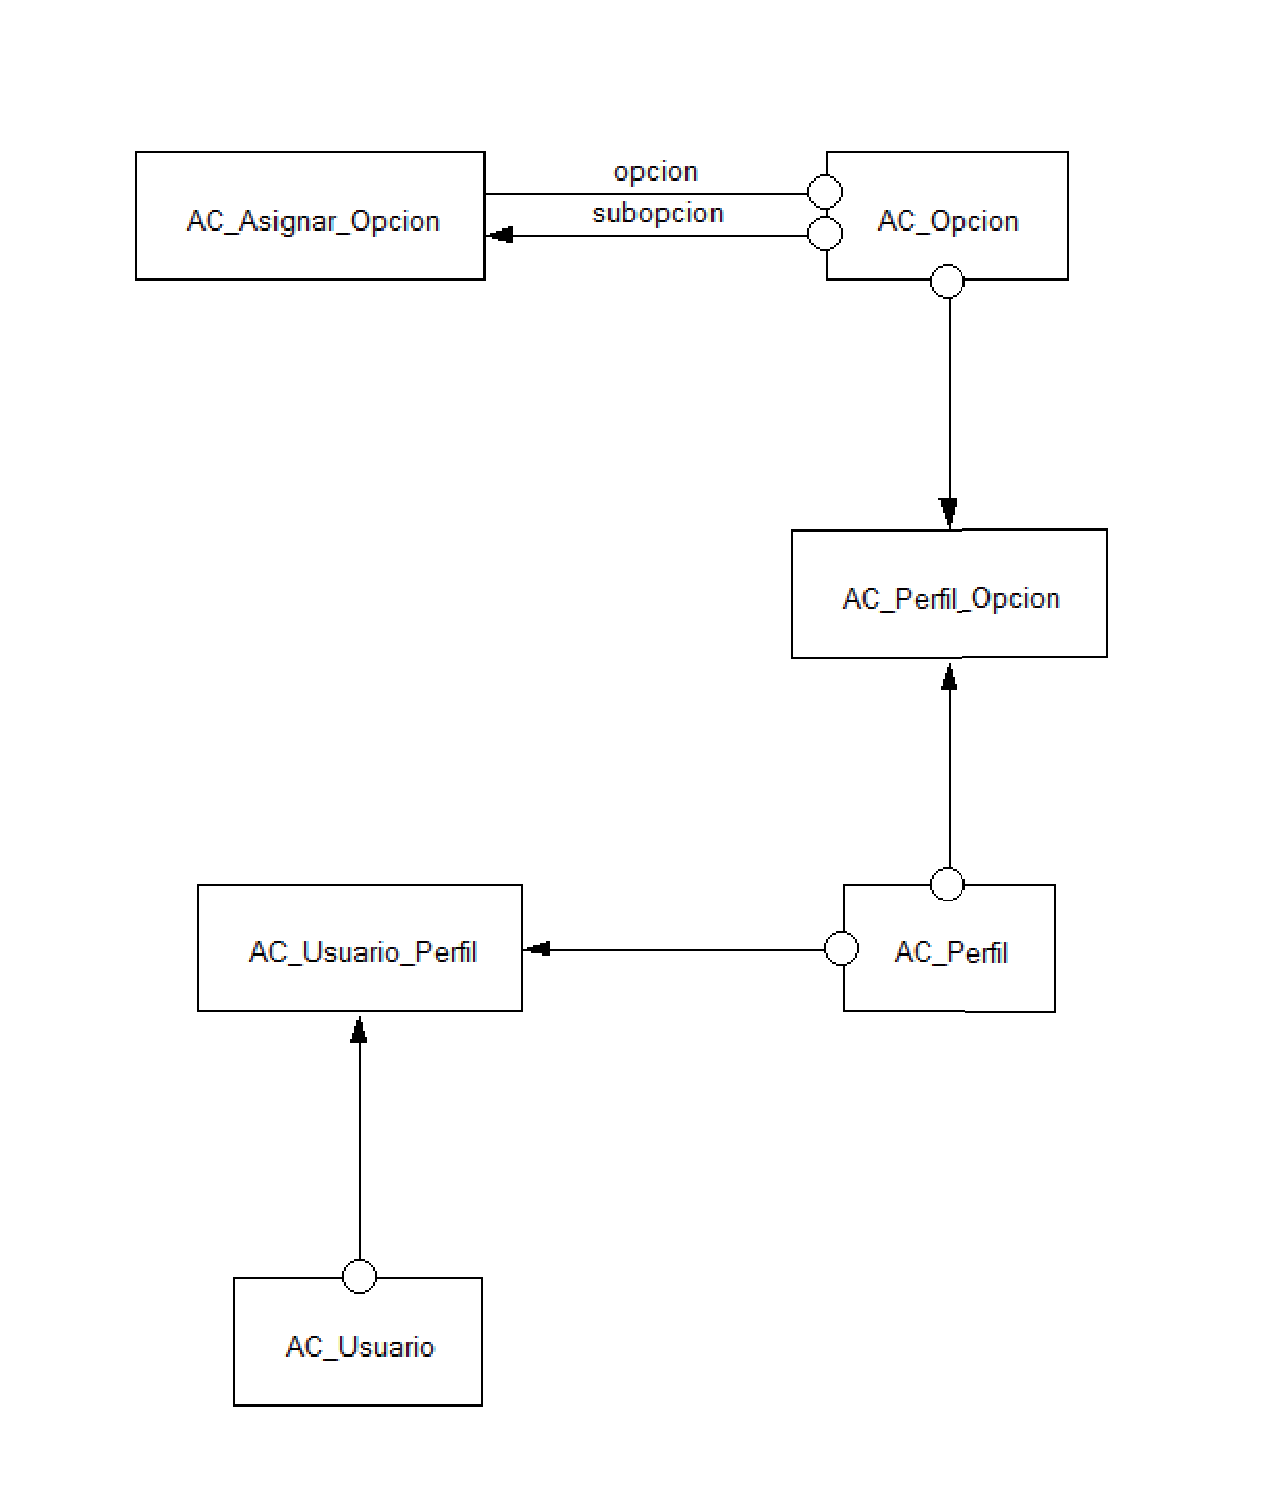
\includegraphics[width=0.5\textwidth]{images/merode-mac.eps}}
  \caption{EDG - M\'odulo de Administraci\'on Central (MAC)}
  \label{edg:mac}
\end{figure}

\textbf{M\'ODULO DE SUSCRIPCI\'ON DE USUARIOS (MSU)}

\textbf{MSU} (\ref{edg:msu}) tiene 8 objetos que se listar\'an a continuaci\'on:

\begin{enumerate}
\item SU\_Titulo
\item SU\_Pais
\item SU\_Ciudad
\item SU\_Empresa
\item SU\_Tipo\_Empresa
\item SU\_Empresa\_Usuario
\item SU\_Tipo\_Empresa\_Cargo
\item SU\_Cargo
\end{enumerate}

En la siguiente ~\ref{diferencias:websae-appvlir8-msu} nos explica las diferencias entre los objetos, dependiendo si es el Sistema actual o el anterior.

\begin{table}
	\begin{center}
	\begin{tabular}{|l|l|p{1.5in}|}
		\hline
		\textbf{WebSAE} & \textbf{AppVlir8} & \textbf{Observaciones} \\
		\hline\hline
		  	SU\_Tipo\_Empresa\_Cargo	&  & Este objeto surgi\'o debido a que anteriormente Cargo depend\'ia de manera directa de Tipo\_Empresa, en la revisi\'on del dise\~no se cambi\'o esa relaci\'on agregando un objeto, de tal manera que ahora Cargo y Tipo de Empresa son independientes. \\
		\hline
	\end{tabular}
	\caption{Diferencias entre los objetos de \textbf{WebSAE} y \textbf{AppVlir8}, en \textbf{MSU}.}\label{diferencias:websae-appvlir8-msu}
	\end{center}
\end{table}

\begin{figure}
  \centering
    {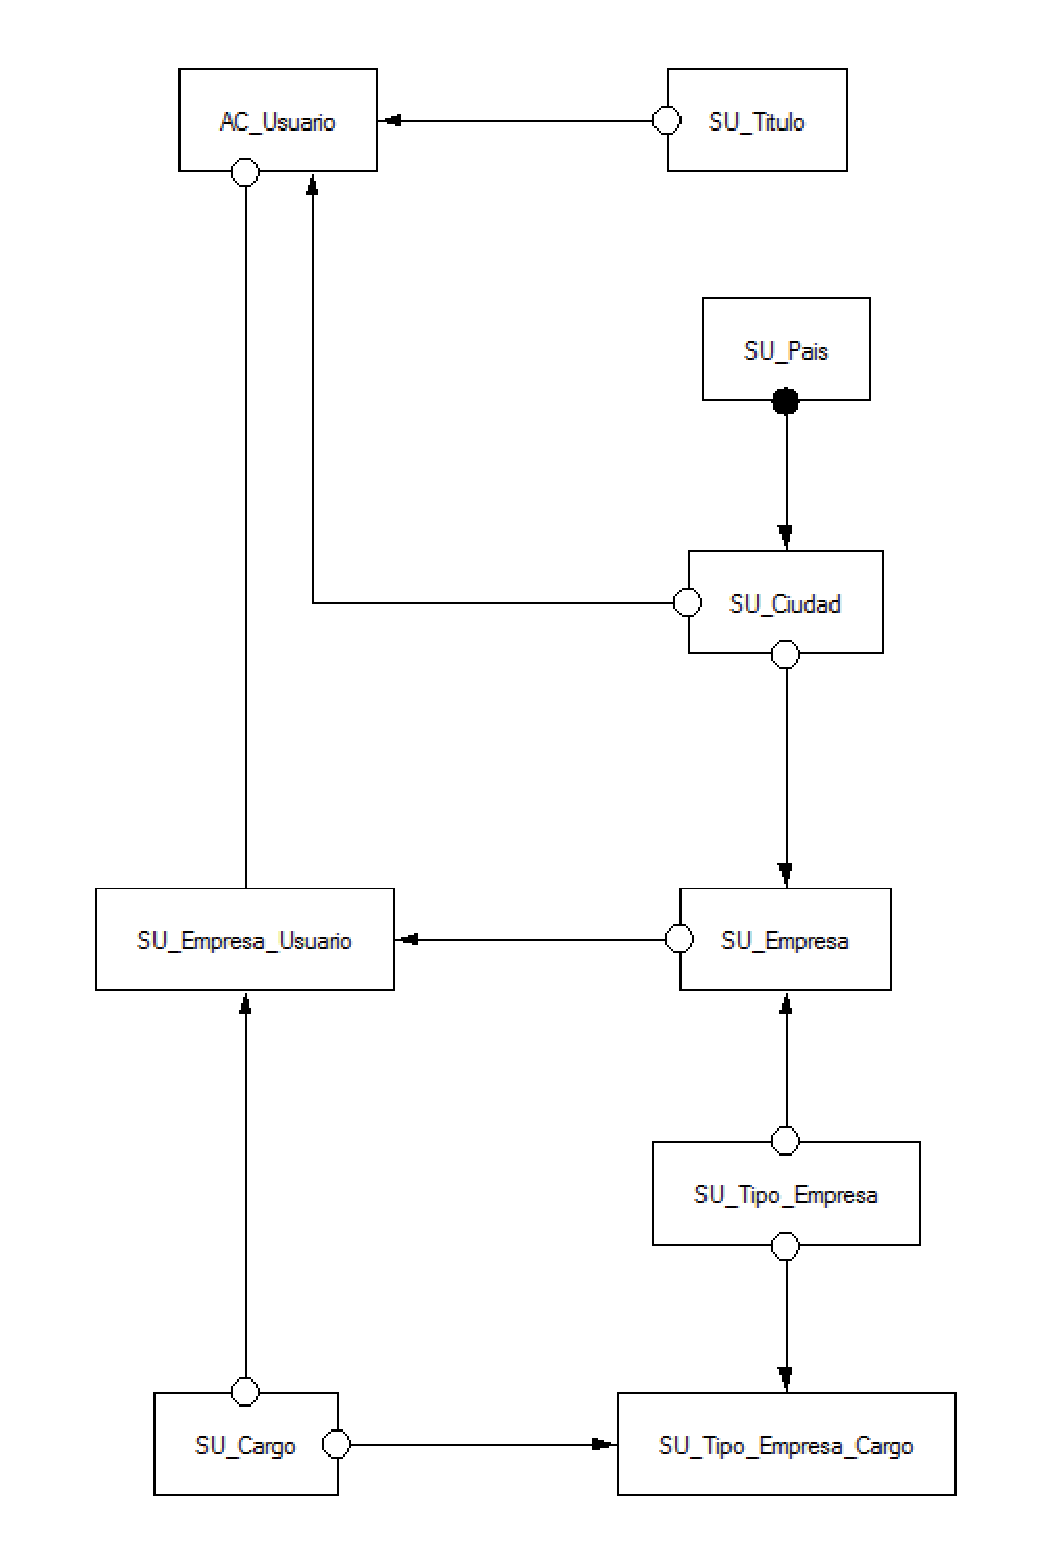
\includegraphics[width=0.5\textwidth]{images/merode-msu.eps}}
  \caption{EDG - M\'odulo de Suscripci\'on de Usuarios (MSU)}
  \label{edg:msu}
\end{figure}

\textbf{M\'ODULO DE ADMINISTRACI\'ON DE EVENTOS (MAE)}

\textbf{MAE} (\ref{edg:mae}) tiene 19 objetos que se listar\'an a continuaci\'on:

\begin{enumerate}
\item AE\_Actividad
\item AE\_Asignar\_Evento
\item AE\_Auspicio
\item AE\_Categoria
\item AE\_Categoria\_Evento
\item AE\_Conferencista\_Evento
\item AE\_Conferencista\_Evento\_Articulo
\item AE\_Evento
\item AE\_Evento\_Opcion
\item AE\_Faq
\item AE\_Fecha\_Evento
\item AE\_Material
\item AE\_Material\_Registro
\item AE\_Organizador
\item AE\_Registro
\item AE\_Subcategoria
\item AE\_Subcategoria\_Evento
\item AE\_Tipo\_Evento
\item AE\_Tipo\_Material
\end{enumerate}

En la siguiente ~\ref{diferencias:websae-appvlir8-mae} nos explica las diferencias entre los objetos, dependiendo si es el Sistema actual o el anterior.

\begin{table}
	\begin{center}
	\begin{tabular}{|p{1.5in}|p{1.5in}|p{1.8in}|}
		\hline
		\textbf{WebSAE} & \textbf{AppVlir8} & \textbf{Observaciones} \\
		\hline\hline
			AE\_Asignar\_Evento & Subevento\_Evento &  \\
		\hline
		  	AE\_Auspicio 		& Auspicio & Adem\'as de la relaci\'on existente con una Empresa, tambi\'en se le agreg\'o la relaci\'on con un Grupo de Investigaci\'on, debido a que tambi\'en pueden ser auspiciantes sin ser los Organizadores. \\
		\hline
		  	AE\_Categoria\_ Evento		& Categoria\_Evento & Es el precio dependiendo de la Categor\'ia. \\
		\hline
		  	AE\_Subcategoria\_ Evento	& Subcategoria\_Evento & Es el porcentaje dependiendo de la Subcategor\'ia. \\
		\hline
		  	AE\_Conferencista\_ Evento	& Conferencista\_Evento & Este objeto en el anterior Sistema estaba en \textbf{MCE}, pero debido a que muchas veces existen conferencistas que son invitados y no necesariamente entran en el proceso de evaluaci\'on de art\'iculos, de ah\'i en la necesidad de cambiar de m\'odulo a este objeto. \\
		\hline
		  	AE\_Conferencista\_ Evento\_Articulo	& AE\_Conferencista\_ Articulo &  \\
		\hline
		  	AE\_Evento\_Opcion						& Menu\_Evento &  \\
		\hline
		  	 & Pregunta\_Faq & Eliminado de WebSAE, debido a que en el objeto Faq, se guardan las preguntas en HTML. \\
		\hline
		  	 & Respuesta\_Faq & Eliminado de WebSAE, por la raz\'on anterior. \\
		\hline
		  	 & Correo & Eliminado de WebSAE. \\
		\hline
	\end{tabular}
	\caption{Diferencias entre los objetos de \textbf{WebSAE} y \textbf{AppVlir8}, en \textbf{MAE}.}\label{diferencias:websae-appvlir8-mae}
	\end{center}
\end{table}

\begin{landscape}
\begin{figure}
  \centering
    {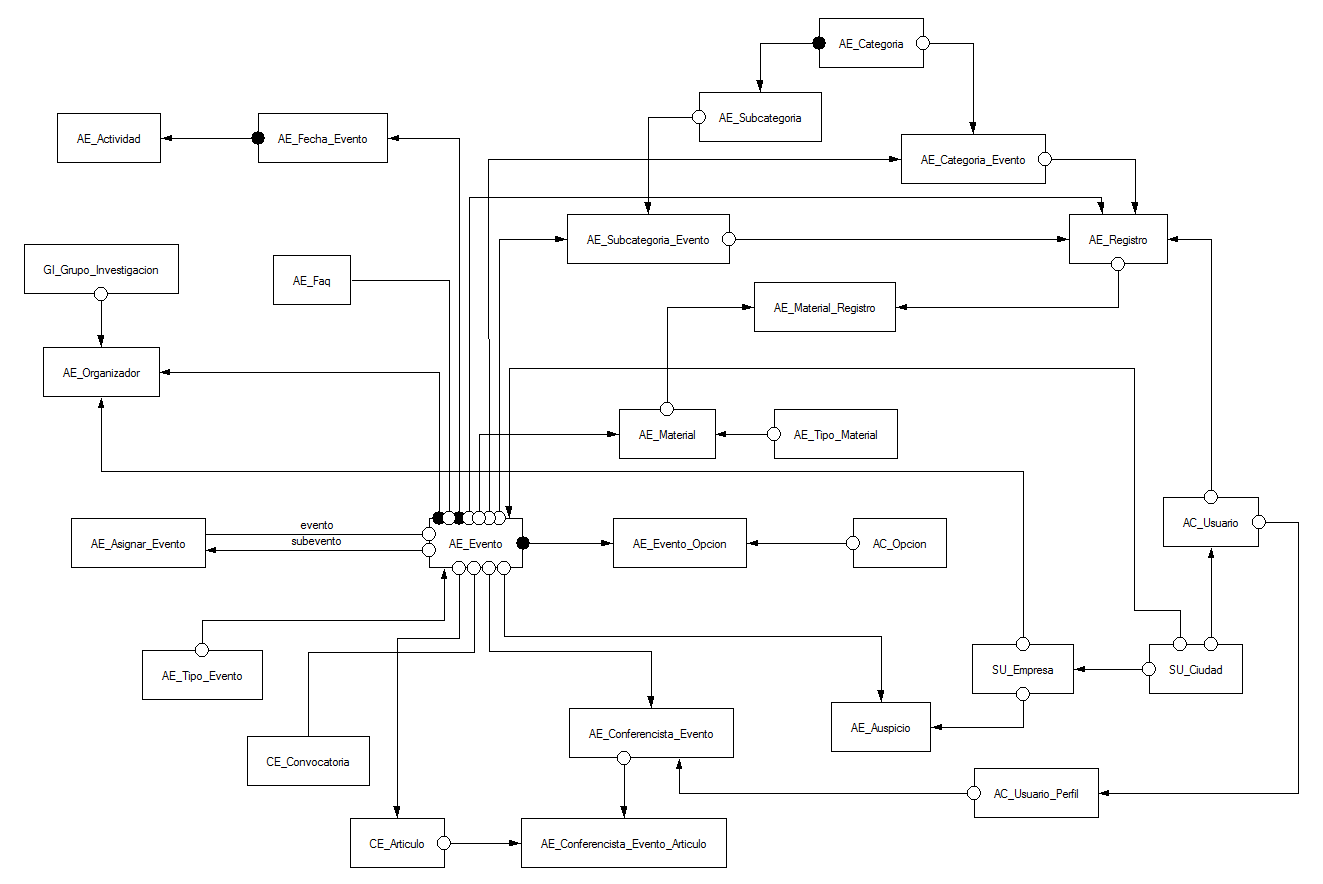
\includegraphics[width=1.1\textwidth]{images/merode-mae.eps}}
  \caption{EDG - M\'odulo de Administraci\'on de Eventos (MAE)}
  \label{edg:mae}
\end{figure}
\end{landscape}

\textbf{M\'ODULO DE CONVOCATORIA Y EVALUACI\'ON DE ART\'ICULOS (MCE)}

\textbf{MCE} (\ref{edg:mce}) tiene 14 objetos que se listar\'an a continuaci\'on:

\begin{enumerate}
\item CE\_Alternativa
\item CE\_Archivo
\item CE\_Articulo
\item CE\_Autor\_Articulo
\item CE\_Convocatoria
\item CE\_Evaluacion
\item CE\_Evaluacion\_Tema\_Articulo
\item CE\_Evaluador\_Articulo
\item CE\_Pregunta
\item CE\_Respuesta
\item CE\_Seccion
\item CE\_Tema
\item CE\_Tema\_Articulo
\item CE\_Tipo\_Pregunta
\end{enumerate}

En la siguiente ~\ref{diferencias:websae-appvlir8-mce} nos explica las diferencias entre los objetos, dependiendo si es el Sistema actual o el anterior.

\begin{table}
	\begin{center}
	\begin{tabular}{|p{1.5in}|p{1.5in}|p{1.8in}|}
		\hline
		\textbf{WebSAE} & \textbf{AppVlir8} & \textbf{Observaciones} \\
		\hline\hline
			CE\_Archivo &  & Agregado debido a que se desea tener todos los archivos que se generen en el proceso de la evaluaci\'on por cada usuario que haya subido su art\'iculo para participar de la convocatoria. \\
		\hline
			CE\_Respuesta & Respuestas & \\
		\hline
			 & Articulo\_Evento & Eliminado de WebSAE, se incluy\'o una relaci\'on directa entre CE\_Evento y CE\_Articulo, en el que CE\_Articulo depende de CE\_Evento. \\
		\hline
	\end{tabular}
	\caption{Diferencias entre los objetos de \textbf{WebSAE} y \textbf{AppVlir8}, en \textbf{MCE}.}\label{diferencias:websae-appvlir8-mce}
	\end{center}
\end{table}

\begin{landscape}
\begin{figure}
  \centering
    {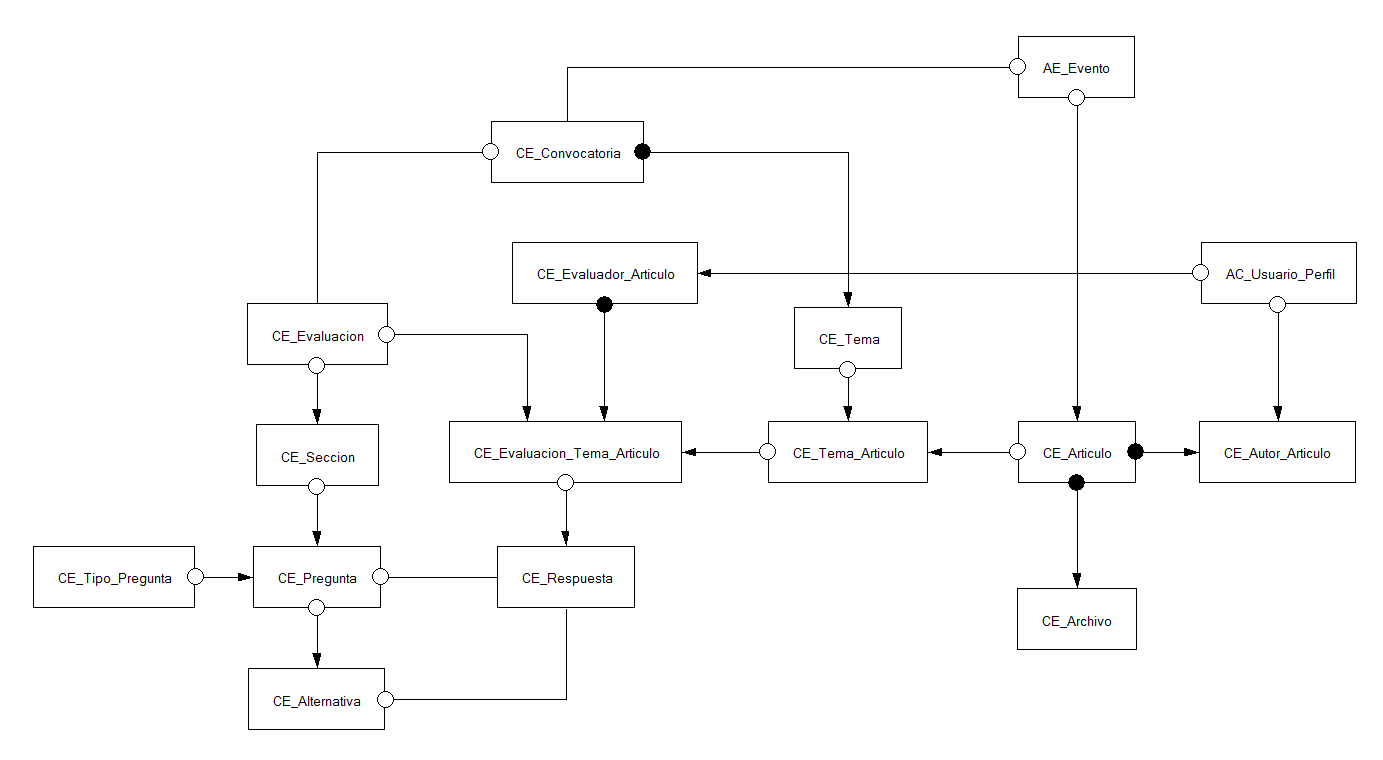
\includegraphics[width=1.3\textwidth]{images/merode-mce.eps}}
  \caption{EDG - M\'odulo de Convocatoria y Evaluaci\'on de Art\'iculos (MCE)}
  \label{edg:mce}
\end{figure}
\end{landscape}
\end{indentar}

\subsection{La tabla de eventos de objetos (OET)}
\begin{indentar}
Para presentar la Tabla de Objetos de Eventos\footnote{Es una matriz que contiene una fila por cada tipo de evento y una columna por cada tipo de objeto, como se ha detallado en el cap\'itulo 2.}, se ha considerado separarla por objetos para que pueda ser apreciada de una mejor manera.

\begin{table}
	\begin{center}
	\begin{tabular}{|r|c|}
		\hline
				& \textbf{AE\_Evento} \\
		\hline\hline
			registrar\_evento	& O/C \\
		\hline
			modificar\_evento	& O/M \\
		\hline
			eliminar\_evento	& O/E \\
		\hline
			registrar\_material	& A/M \\
		\hline
			modificar\_material	& A/M \\
		\hline
			eliminar\_material	& A/M \\
		\hline
			registrar\_material\_subevento	& A/M \\
		\hline
			modificar\_material\_subevento	& A/M \\
		\hline
			eliminar\_material\_subevento	& A/M \\
		\hline
			asignar\_evento\_opcion	& A/M \\
		\hline
			actualizar\_faq	& A/M \\
		\hline
			registrar\_agenda	& A/M \\
		\hline
			modificar\_agenda	& A/M \\
		\hline
			eliminar\_agenda	& A/M \\
		\hline
			registrar\_auspiciante	& A/M \\
		\hline
			modificar\_auspiciante	& A/M \\
		\hline
			eliminar\_auspiciante	& A/M \\
		\hline
			registrar\_horario	& A/M \\
		\hline
			modificar\_horario	& A/M \\
		\hline
			eliminar\_horario	& A/M \\
		\hline
			registrar\_subcategoria	& A/M \\
		\hline
			modificar\_subcategoria	& A/M \\
		\hline
			eliminar\_subcategoria	& A/M \\
		\hline
			registrar\_subcategoria\_evento	& A/M \\
		\hline
			modificar\_subcategoria\_evento	& A/M \\
		\hline
			eliminar\_subcategoria\_evento	& A/M \\
		\hline
			registrar\_subcategoria\_subevento	& A/M \\
		\hline
			modificar\_subcategoria\_subevento	& A/M \\
		\hline
			eliminar\_subcategoria\_subevento	& A/M \\
		\hline
			registrar\_categoria\_evento	& A/M \\
		\hline
			modificar\_categoria\_evento	& A/M \\
		\hline
			eliminar\_categoria\_evento	& A/M \\
		\hline
			registrar\_categoria\_subevento	& A/M \\
		\hline
			modificar\_categoria\_subevento	& A/M \\
		\hline
			eliminar\_categoria\_subevento	& A/M \\
		\hline
			registrar\_conferencista\_evento	& A/M \\
		\hline
			modificar\_conferencista\_evento	& A/M \\
		\hline
			eliminar\_conferencista\_evento	& A/M \\
		\hline
			registrar\_conferencista\_subevento	& A/M \\
		\hline
			modificar\_conferencista\_subevento	& A/M \\
		\hline
			eliminar\_conferencista\_subevento	& A/M \\
		\hline
	\end{tabular}
	\caption{OET - Objeto AE\_Evento (Parte 1)}
	\label{oet:evento}
	\end{center}
\end{table}

\begin{table}
	\begin{center}
	\begin{tabular}{|r|c|}
		\hline
				& \textbf{AE\_Evento} \\
		\hline\hline
			registrar\_organizador	& A/M \\
		\hline
			eliminar\_organizador	& A/M \\
		\hline
			registrar\_subevento	& O/C \\
		\hline
			modificar\_subevento	& O/M \\
		\hline
			eliminar\_subevento	& O/E \\
		\hline
			registrar\_usuario\_evento	& A/M \\
		\hline
			eliminar\_usuario\_evento	& A/M \\
		\hline
	\end{tabular}
	\caption{OET - Objeto AE\_Evento (Parte 2)}
	\label{oet:evento}
	\end{center}
\end{table}

\end{indentar}

\subsection{M\'aquina de estados finitos relevantes (FSM)}
\begin{indentar}

\begin{figure}
  \centering
    {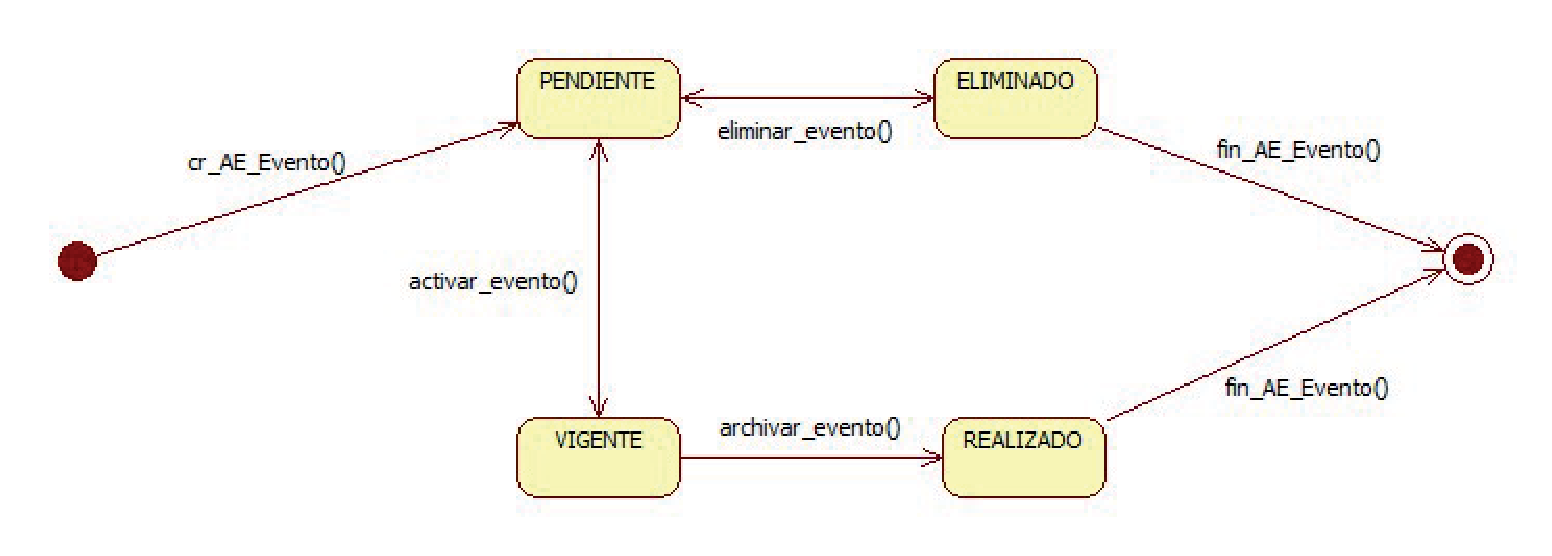
\includegraphics[width=1.0\textwidth]{images/estado-evento.eps}}
  \caption{FSM - Estados del Objeto AE\_Evento}
  \label{estados:ae_evento}
\end{figure}

\begin{figure}
  \centering
    {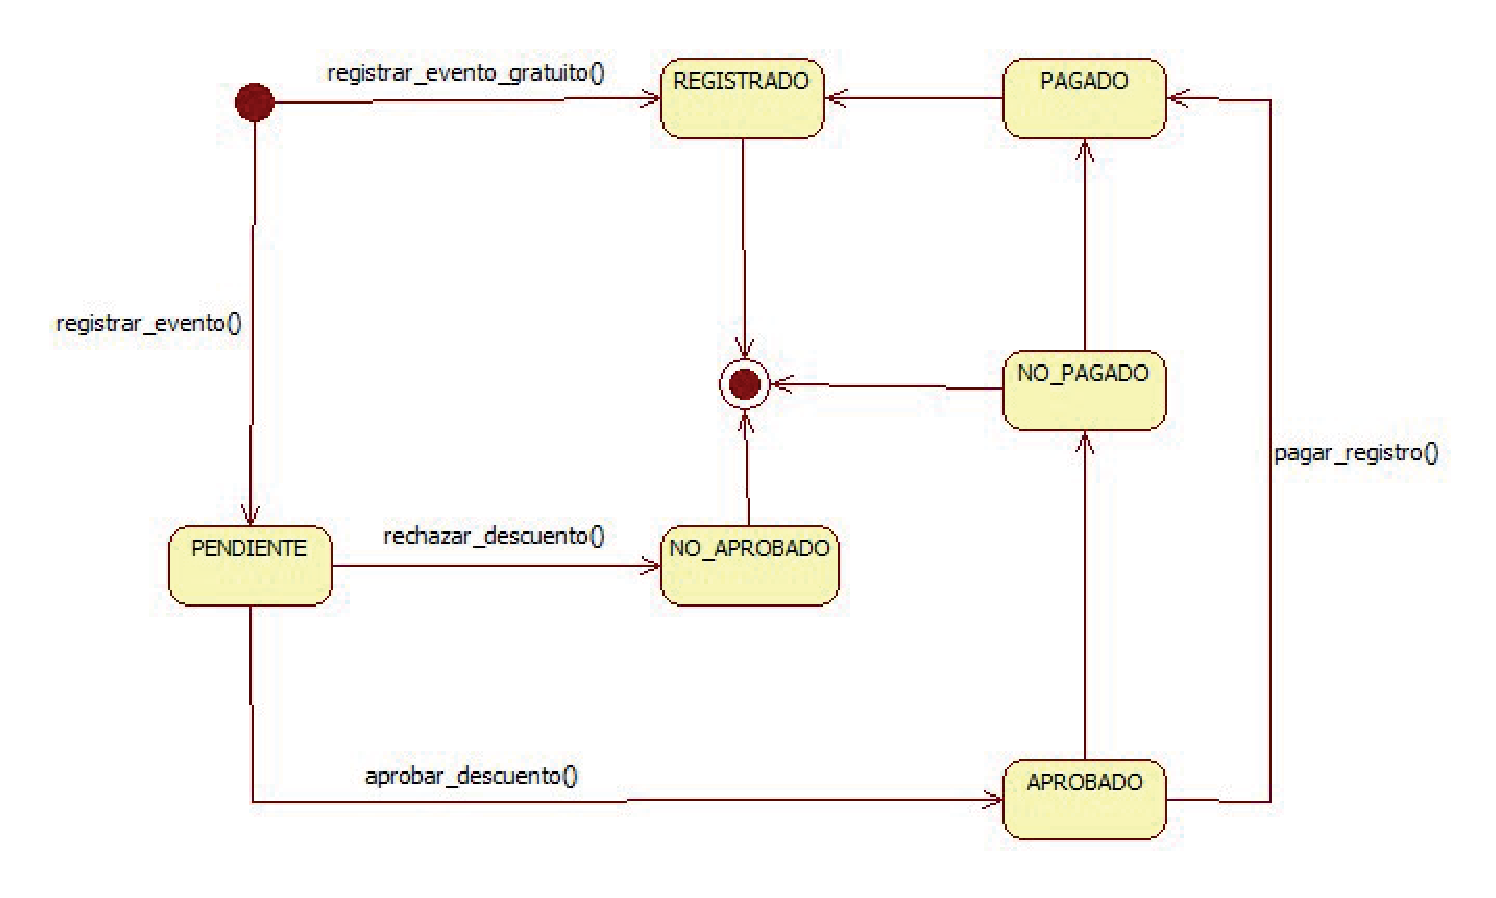
\includegraphics[width=1.0\textwidth]{images/estado-registro.eps}}
  \caption{FSM - Estados del Objeto AE\_Registro}
  \label{estados:ae_registro}
\end{figure}

\end{indentar}

\section{Definici\'on del Modelo espec\'ifico de la plataforma (PSM)}
\begin{indentar}
Luego de elaborar el correspondiente EDG, se pas\'o a la etapa del PSM, el cual fue diagramado mediante una herramienta Open Source, llamada StarUML\footnote{\url{http://staruml.sourceforge.net/en/}}.

Los m\'odulos del PIM anterior tan s\'olo fueron pasados al simil en UML, para su correspondiente transformaci\'on al c\'odigo, en el momento debido.
\begin{landscape}
\begin{figure}
  \centering
    {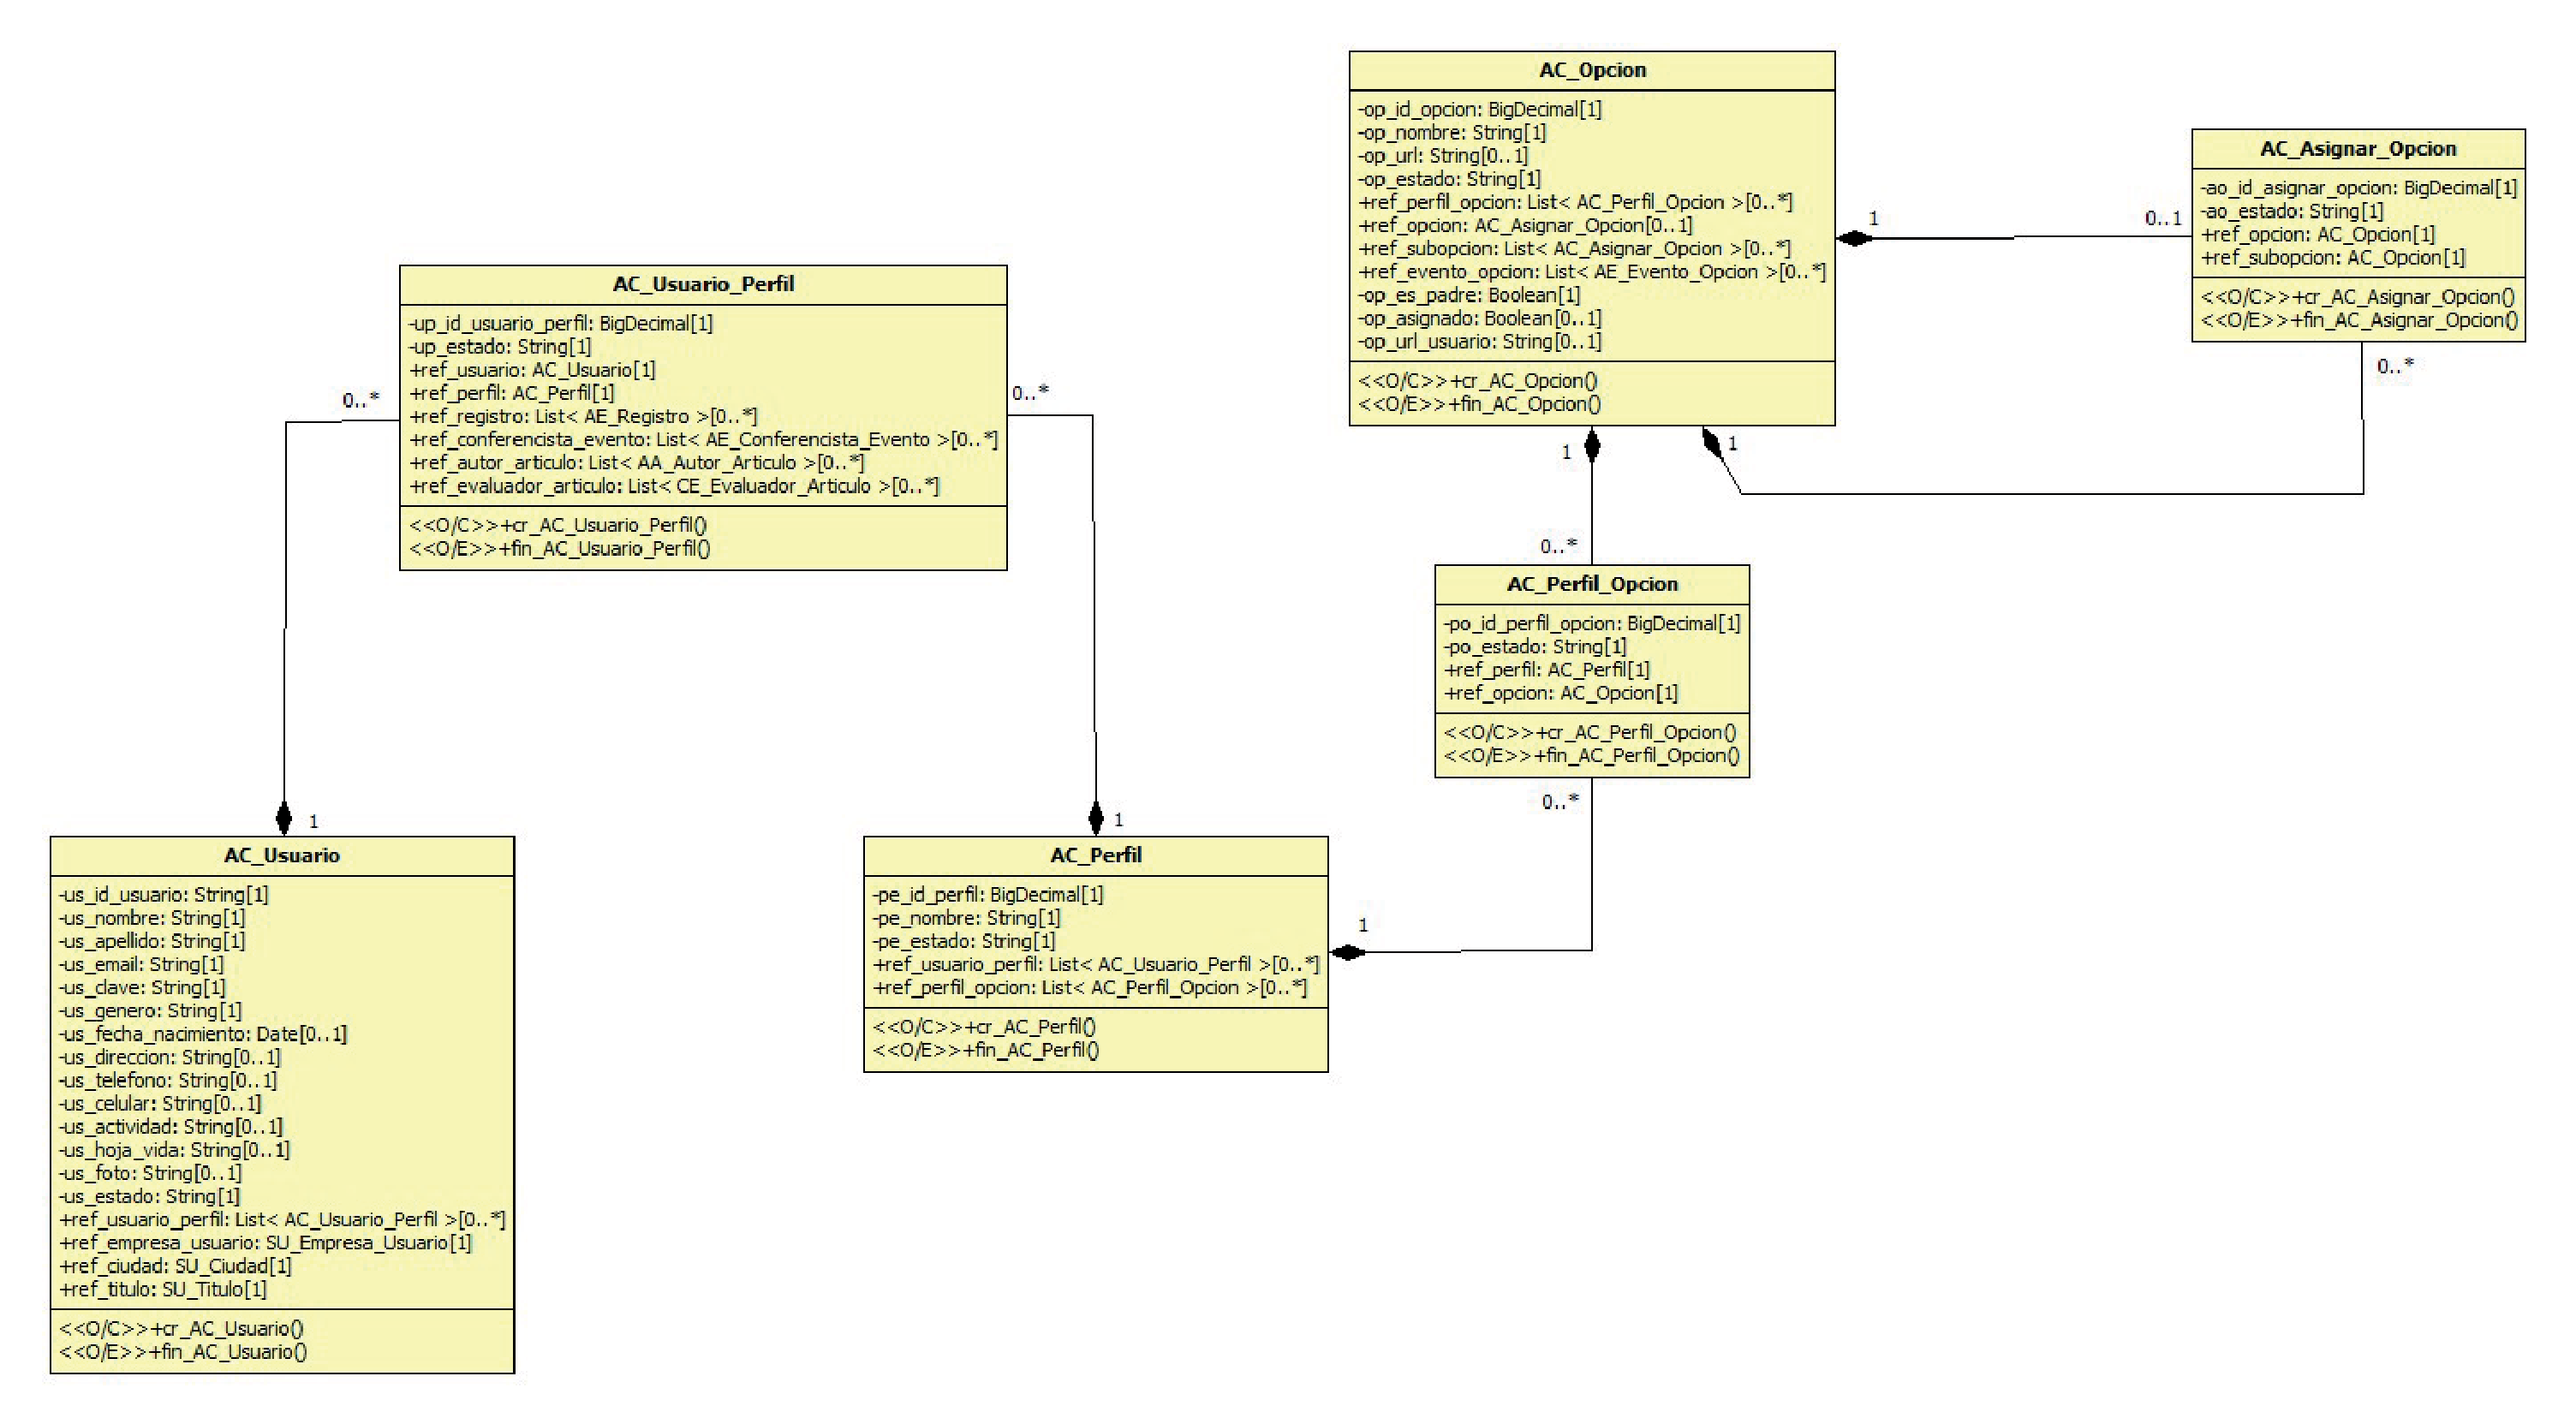
\includegraphics[width=1.7\textwidth]{images/uml-mac.eps}}
  \caption{UML - M\'odulo de Administraci\'on Central (MAC)}
  \label{uml:mac}
\end{figure}
\end{landscape}

\begin{landscape}
\begin{figure}
  \centering
    {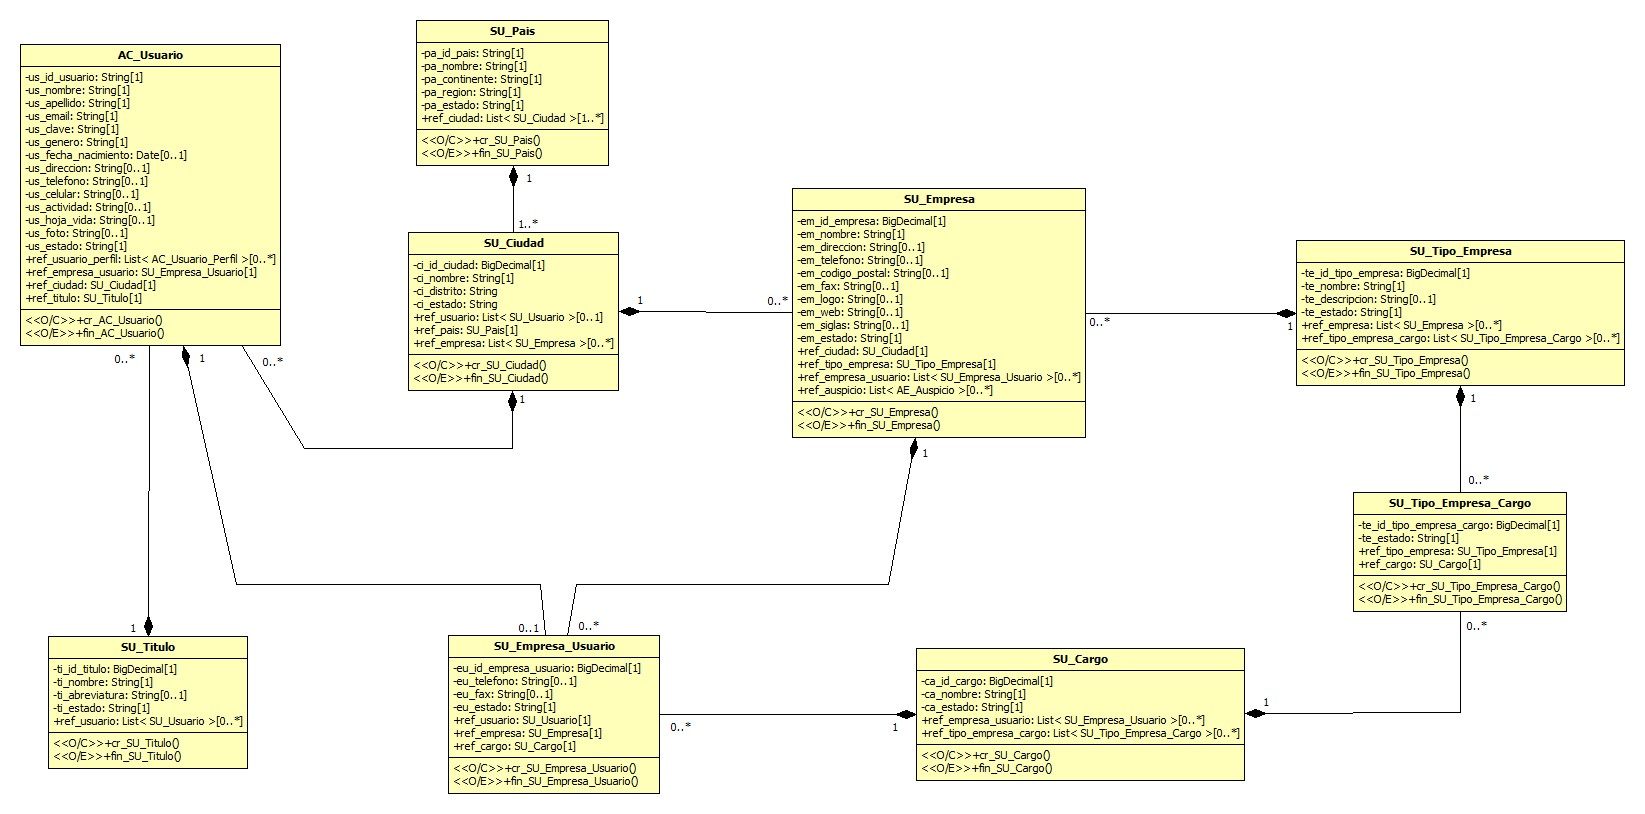
\includegraphics[width=1.7\textwidth]{images/uml-msu.eps}}
  \caption{UML - M\'odulo de Suscripci\'on de Usuarios (MSU)}
  \label{uml:msu}
\end{figure}
\end{landscape}

\begin{landscape}
\begin{figure}
  \centering
    {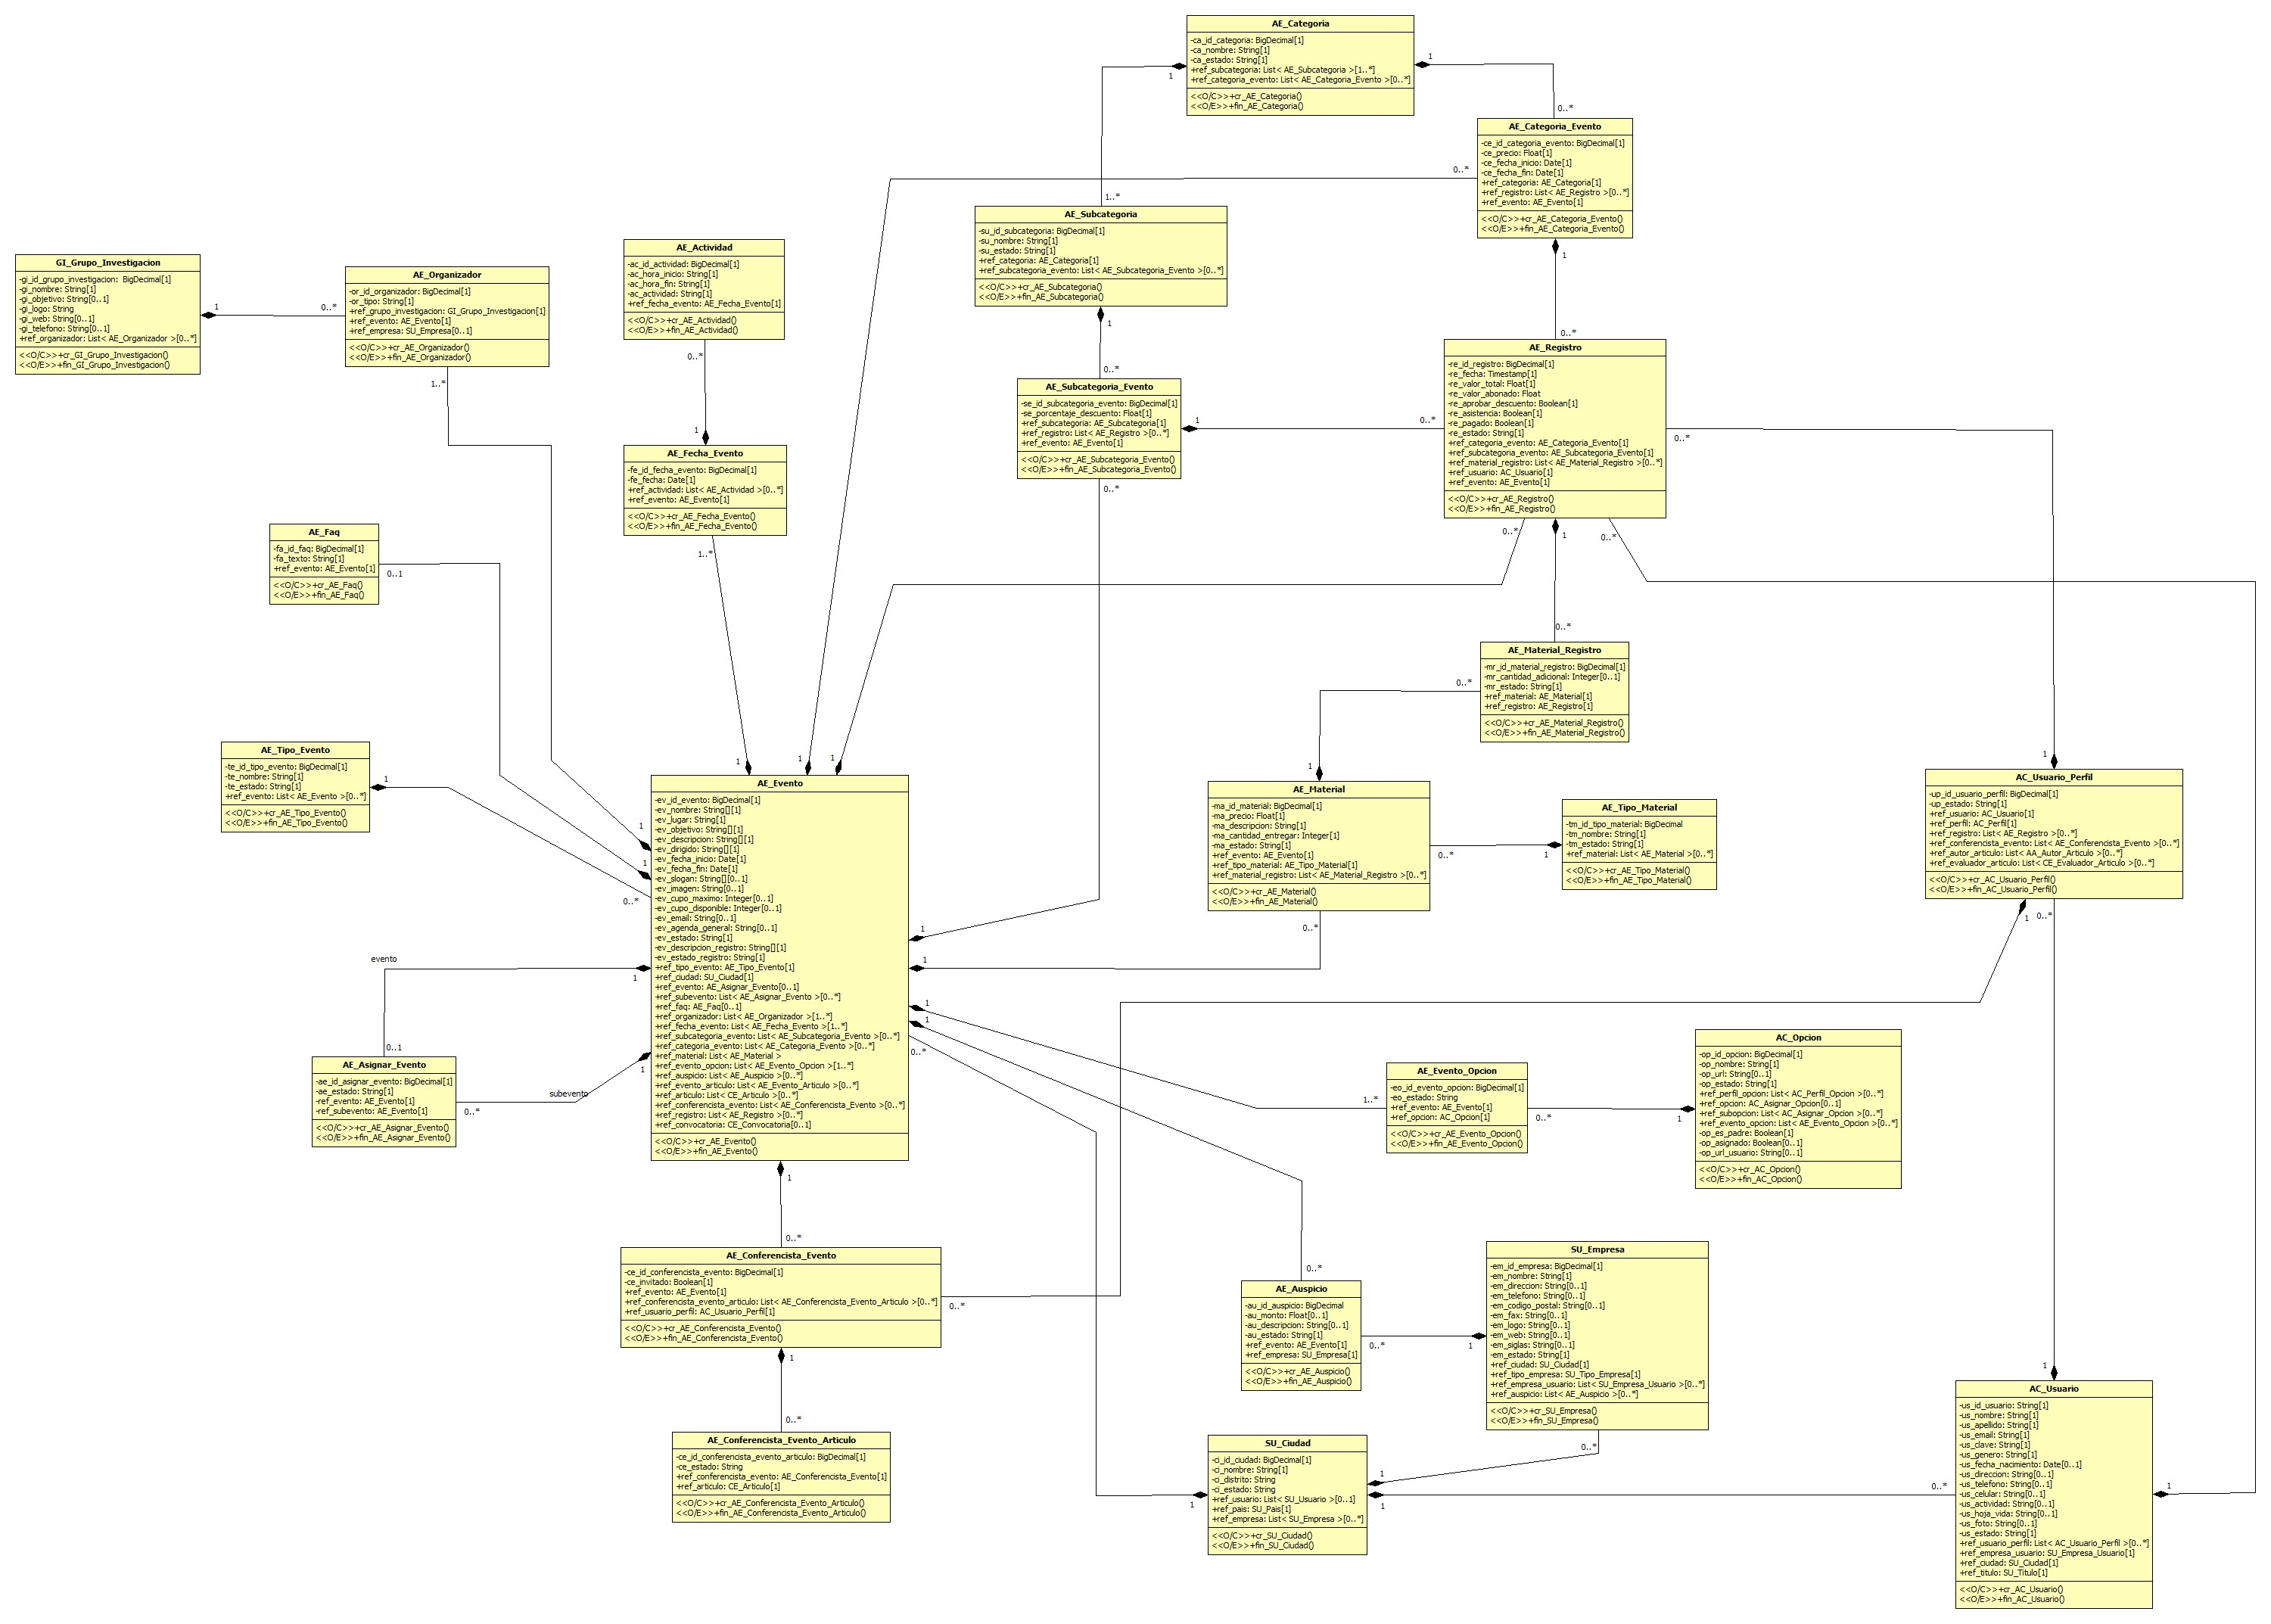
\includegraphics[width=1.3\textwidth]{images/uml-mae.eps}}
  \caption{UML - M\'odulo de Administraci\'on de Eventos (MAE)}
  \label{uml:mae}
\end{figure}
\end{landscape}

\begin{landscape}
\begin{figure}
  \centering
    {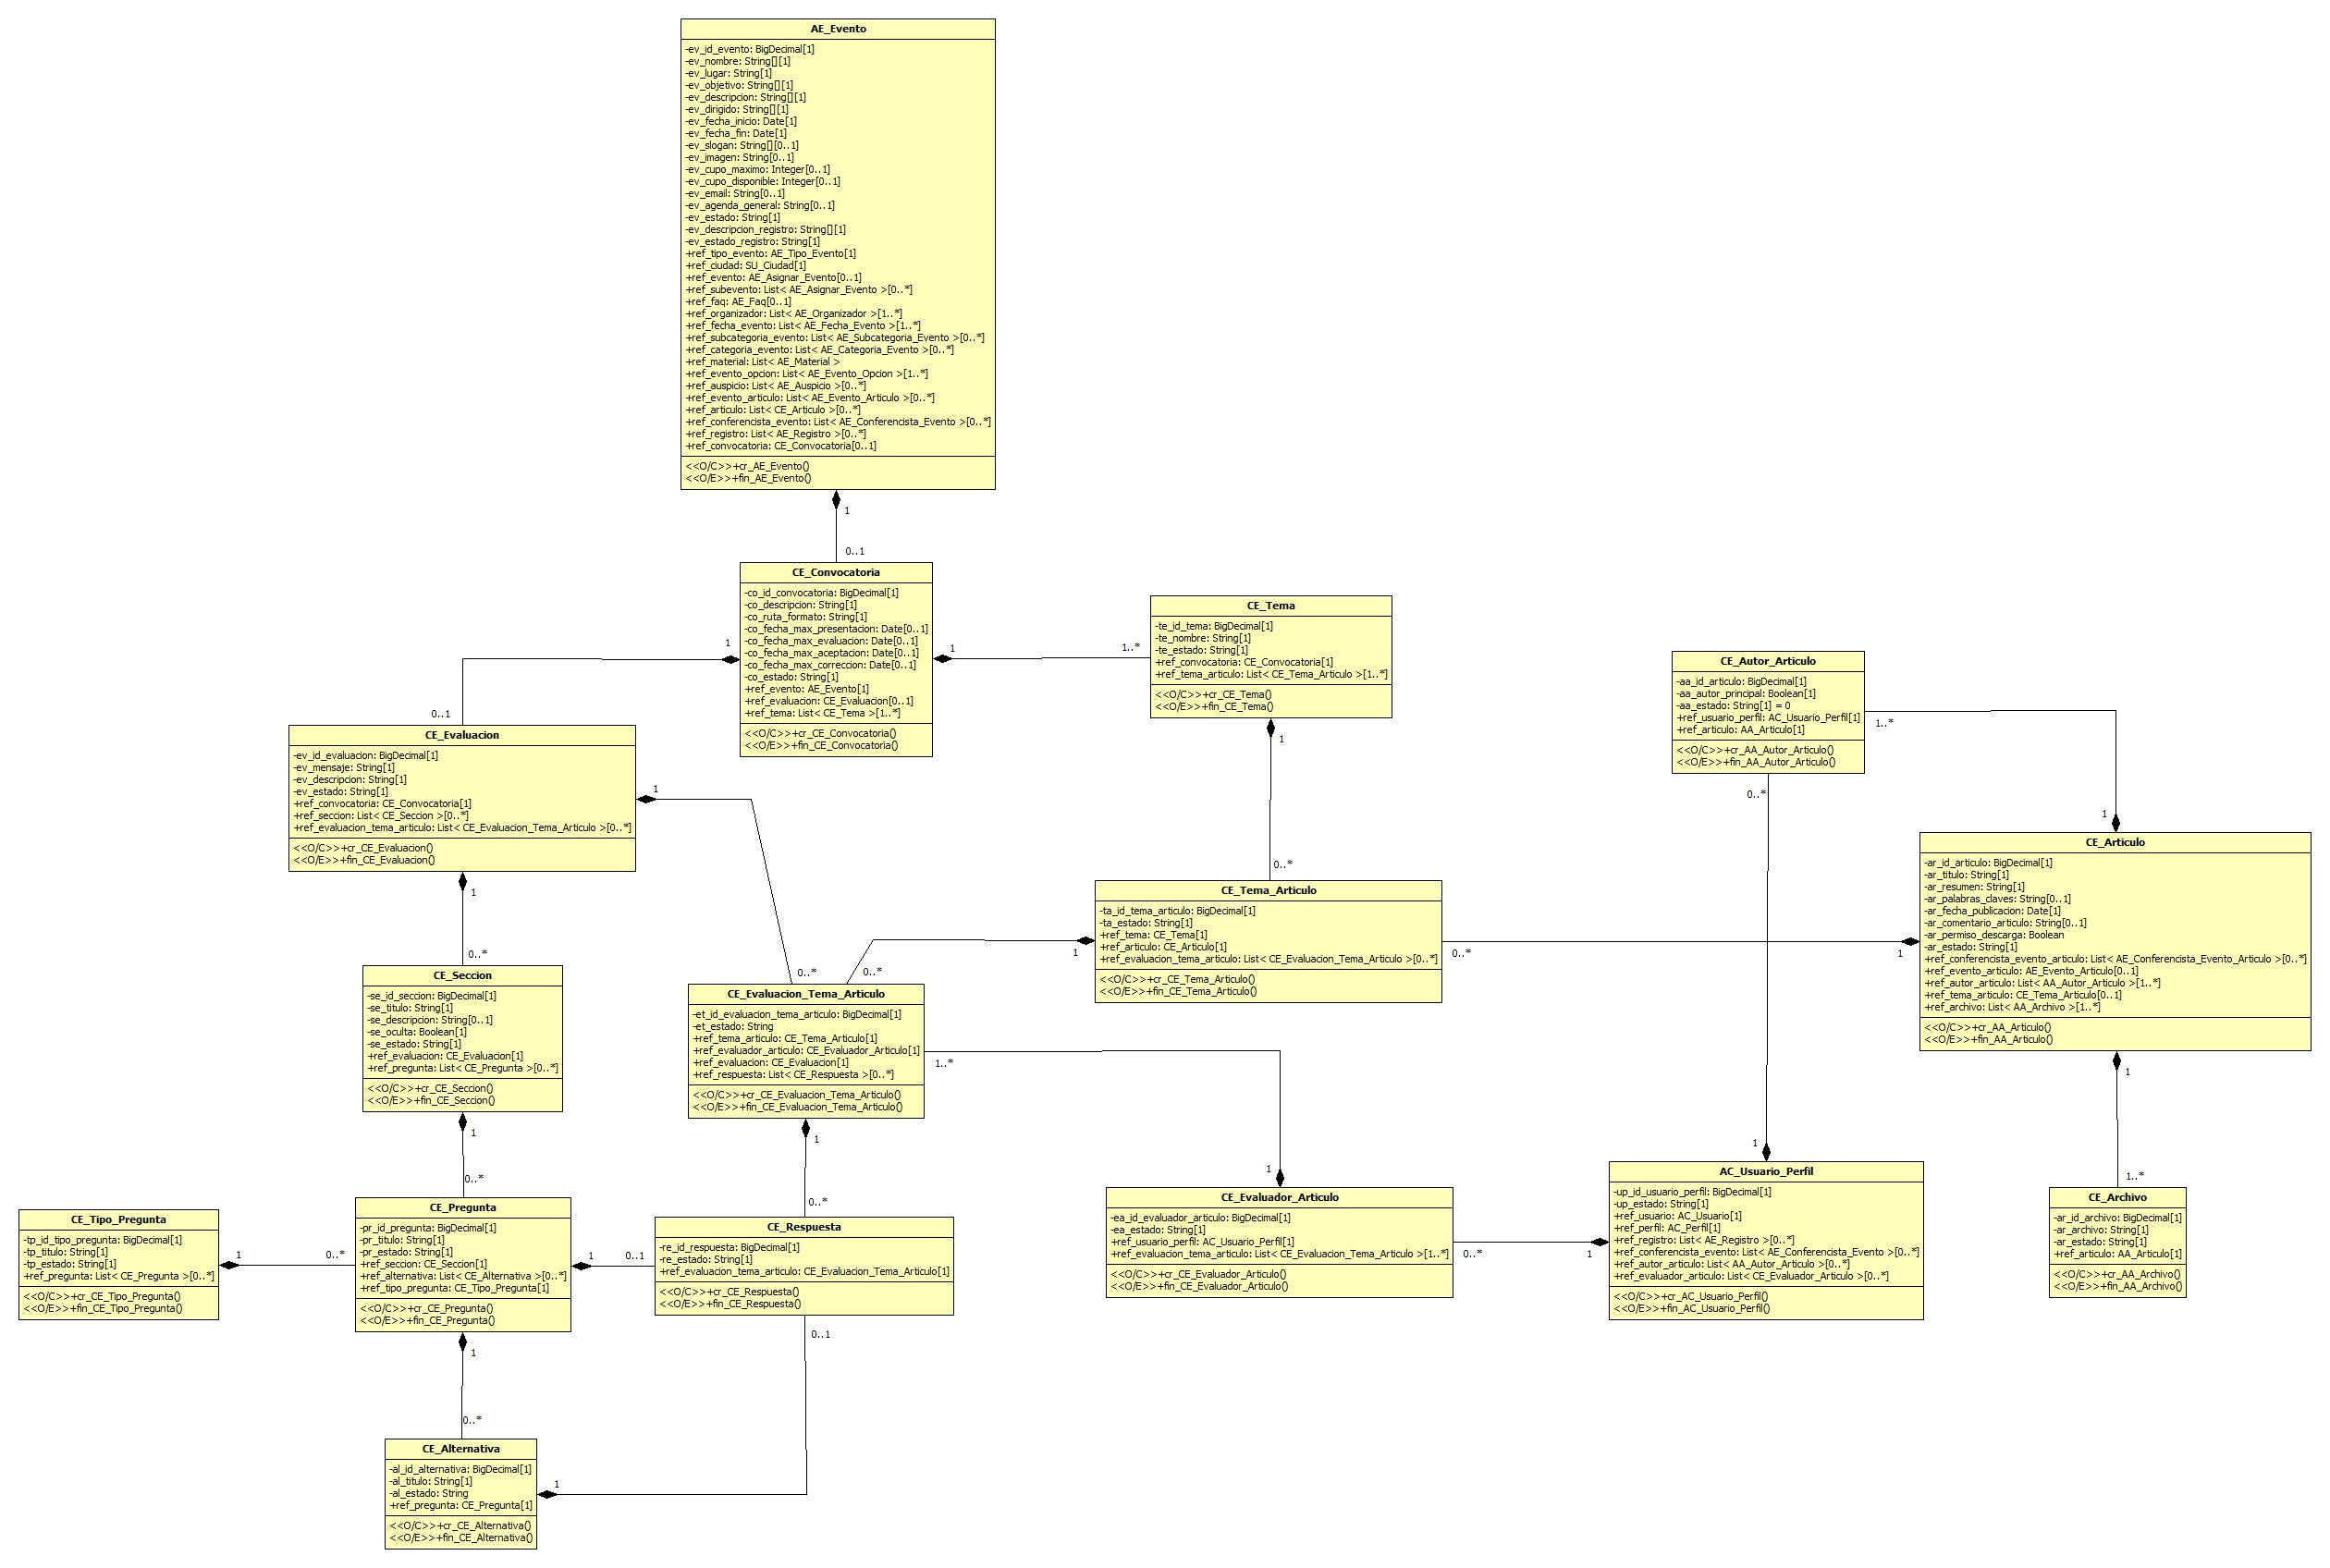
\includegraphics[width=1.5\textwidth]{images/uml-mce.eps}}
  \caption{UML - M\'odulo de Convocatoria y Evaluaci\'on de Art\'iculos (MCE)}
  \label{uml:mce}
\end{figure}
\end{landscape}

\end{indentar}

\section{Definici\'on de Roles en los M\'odulos}
\begin{indentar}
En la siguiente tabla~\ref{usuario:rol}, se muestran las funciones que ejerce cada usuario de un Grupo de Investigaci\'on desde el punto de vista de los acontecimientos del evento y desde el punto de vista del Sistema.

Cada usuario registrado en el Sistema, tiene la posibilidad de tener de uno o m\'as perfiles, de tal manera que pueden ejercer varios roles, dependiendo de las pol\'iticas especificadas por el Comit\'e Organizador.
\begin{table}
	\begin{center}
	\begin{tabular}{|p{1.5in}|p{2.2in}|p{1.5in}|}
		\hline
		\textbf{Usuario} & \textbf{Funci\'on dentro del negocio} & \textbf{Funci\'on dentro del Sistema} \\
		\hline\hline
		Director del Grupo de Investigaci\'on  	& Representante del Grupo de Investigaci\'on, encargado de planificar y elaborar las directrices para los dem\'as miembros organizadores, con la finalidad de llevar a cabo un evento de \'ambito cient\'ifico. & Administrador General \\
		\hline
		Consejo T\'ecnico Organizador		   		& Consejo conformado por los organizadores, una de sus tareas es la de decidir qu\'e resumen de un art\'iculo cient\'ifico -presentado por los posibles conferencistas- es v\'alido para darle paso al siguiente proceso de evaluaci\'on. & Administrador \\
		\hline
		Asistente del Grupo de Investigaci\'on		& Ayudante del Director del centro que sigue las directrices planificadas para la elaboraci\'on exitosa del evento.

Cabe recalcar que el asistente tiene un perfil igual al del Director, s\'olo por razones pr\'acticas. & Administrador General \\
		\hline
		Suscriptor					 						& Usuario visitante del Portal con la finalidad de estar vinculado con un Grupo de Investigaci\'on o por el deseo de registrarse a un evento.  & Suscriptor \\
		\hline
		Evaluador											& Participante del evento en calidad de evaluador, con el prop\'osito de verificar la utilidad del conocimiento demostrado en el art\'iculo. & Evaluador \\
		\hline
		Conferencista										& Usuario que present\'o un art\'iculo de \'indole cient\'ifico con un resultado exitoso, el conferencista tambi\'en puede ser invitado por el Comit\'e Organizador. & Conferencista \\
		\hline
	\end{tabular}
	\caption{Definici\'on de Roles en los M\'odulos}\label{usuario:rol}
	\end{center}
\end{table}
\end{indentar}

\chapter{Dise\~no del Sistema}
\begin{indentar}
\end{indentar}

\section{Dise\~no de la Arquitectura del Sistema}
\begin{indentar}
Debido al requerimiento no funcional, de separar el Sistema actual \textbf{AppVlir8} en dos productos, uno en la Administraci\'on de Eventos Cient\'ificos y el otro en la Administraci\'on de Grupos de Investigaci\'on, el dise\~no de la Arquitectura fue concebido de la siguiente manera.

\begin{figure}
  \centering
    {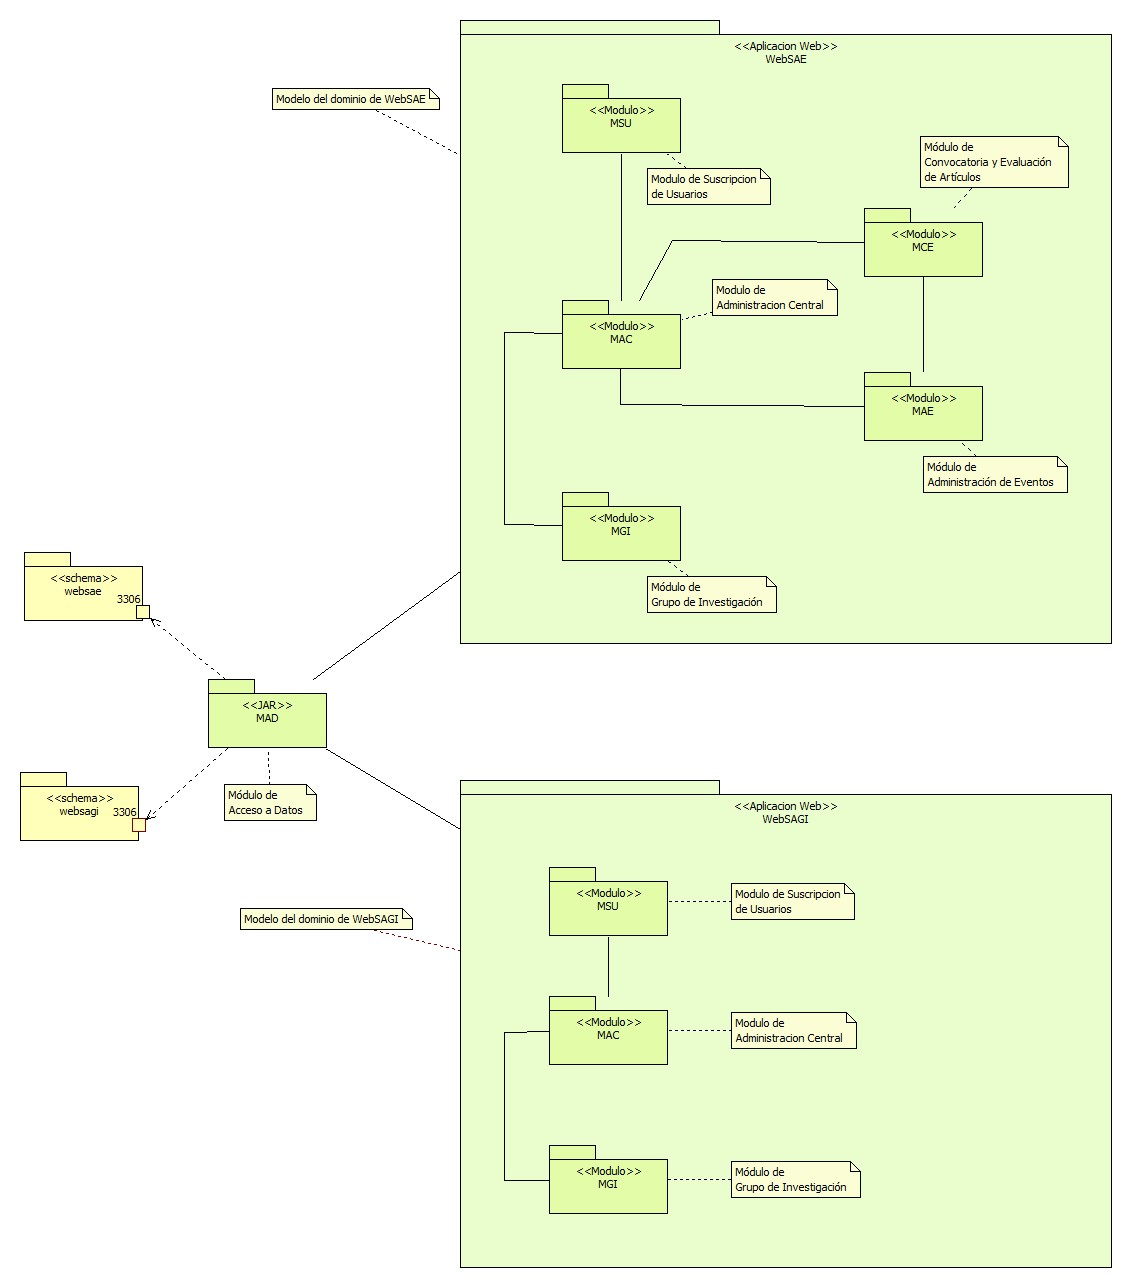
\includegraphics[width=1.0\textwidth]{images/websaegi-arquitectura.eps}}
  \caption{Dise\~no de Arquitectura del Sistema de Administraci\'on de Eventos y Grupos Cient\'ificos.}
  \label{websaegi:arquitectura}
\end{figure}

La definici\'on de la anterior imagen~\ref{websaegi:arquitectura}, es concebida como dos sistemas independientes que utilizan otro m\'odulo no mencionado al inicio, debido a que este m\'odulo no pertenece al dominio, si no que surge en el dise\~no de la Arquitectura, este m\'odulo fue llamado MAD (M\'odulo de Acceso a Datos)\footnote{Es importante recalcar que este m\'odulo fue ideado por la Srta. Diana Crespo -jefa de Sistemas en Molemotor-, llam\'andolo inicialmente ADA, por el dise\~no portable de \'este, se lo adecu\'o a MySQL -ya que fue implementado para que trabajase con la Base de Datos SQL Server 2000- y para que pueda trabajar con WebSAE y WebSAGI, las bases de datos de la Administraci\'on de Eventos y de los Grupos de Investigaci\'on, respectivamente.} este framework, permite a los Eventos la conexi\'on a la Base de Datos de los Grupos de Investigaci\'on y viceverza.
\end{indentar}

\subsection{Dise\~no Arquitect\'onico}
\begin{indentar}
En nuestro caso, s\'olo se implement\'o el Sistema Web de Administraci\'on de Eventos Cient\'ificos, tambi\'en denominado \textbf{WebSAE}, el mismo que se muestra a continuaci\'on \ref{websae:arquitectura}, que ser\'ia tan s\'olo una de las partes antes mostrada.

\begin{landscape}
\begin{figure}
  \centering
    {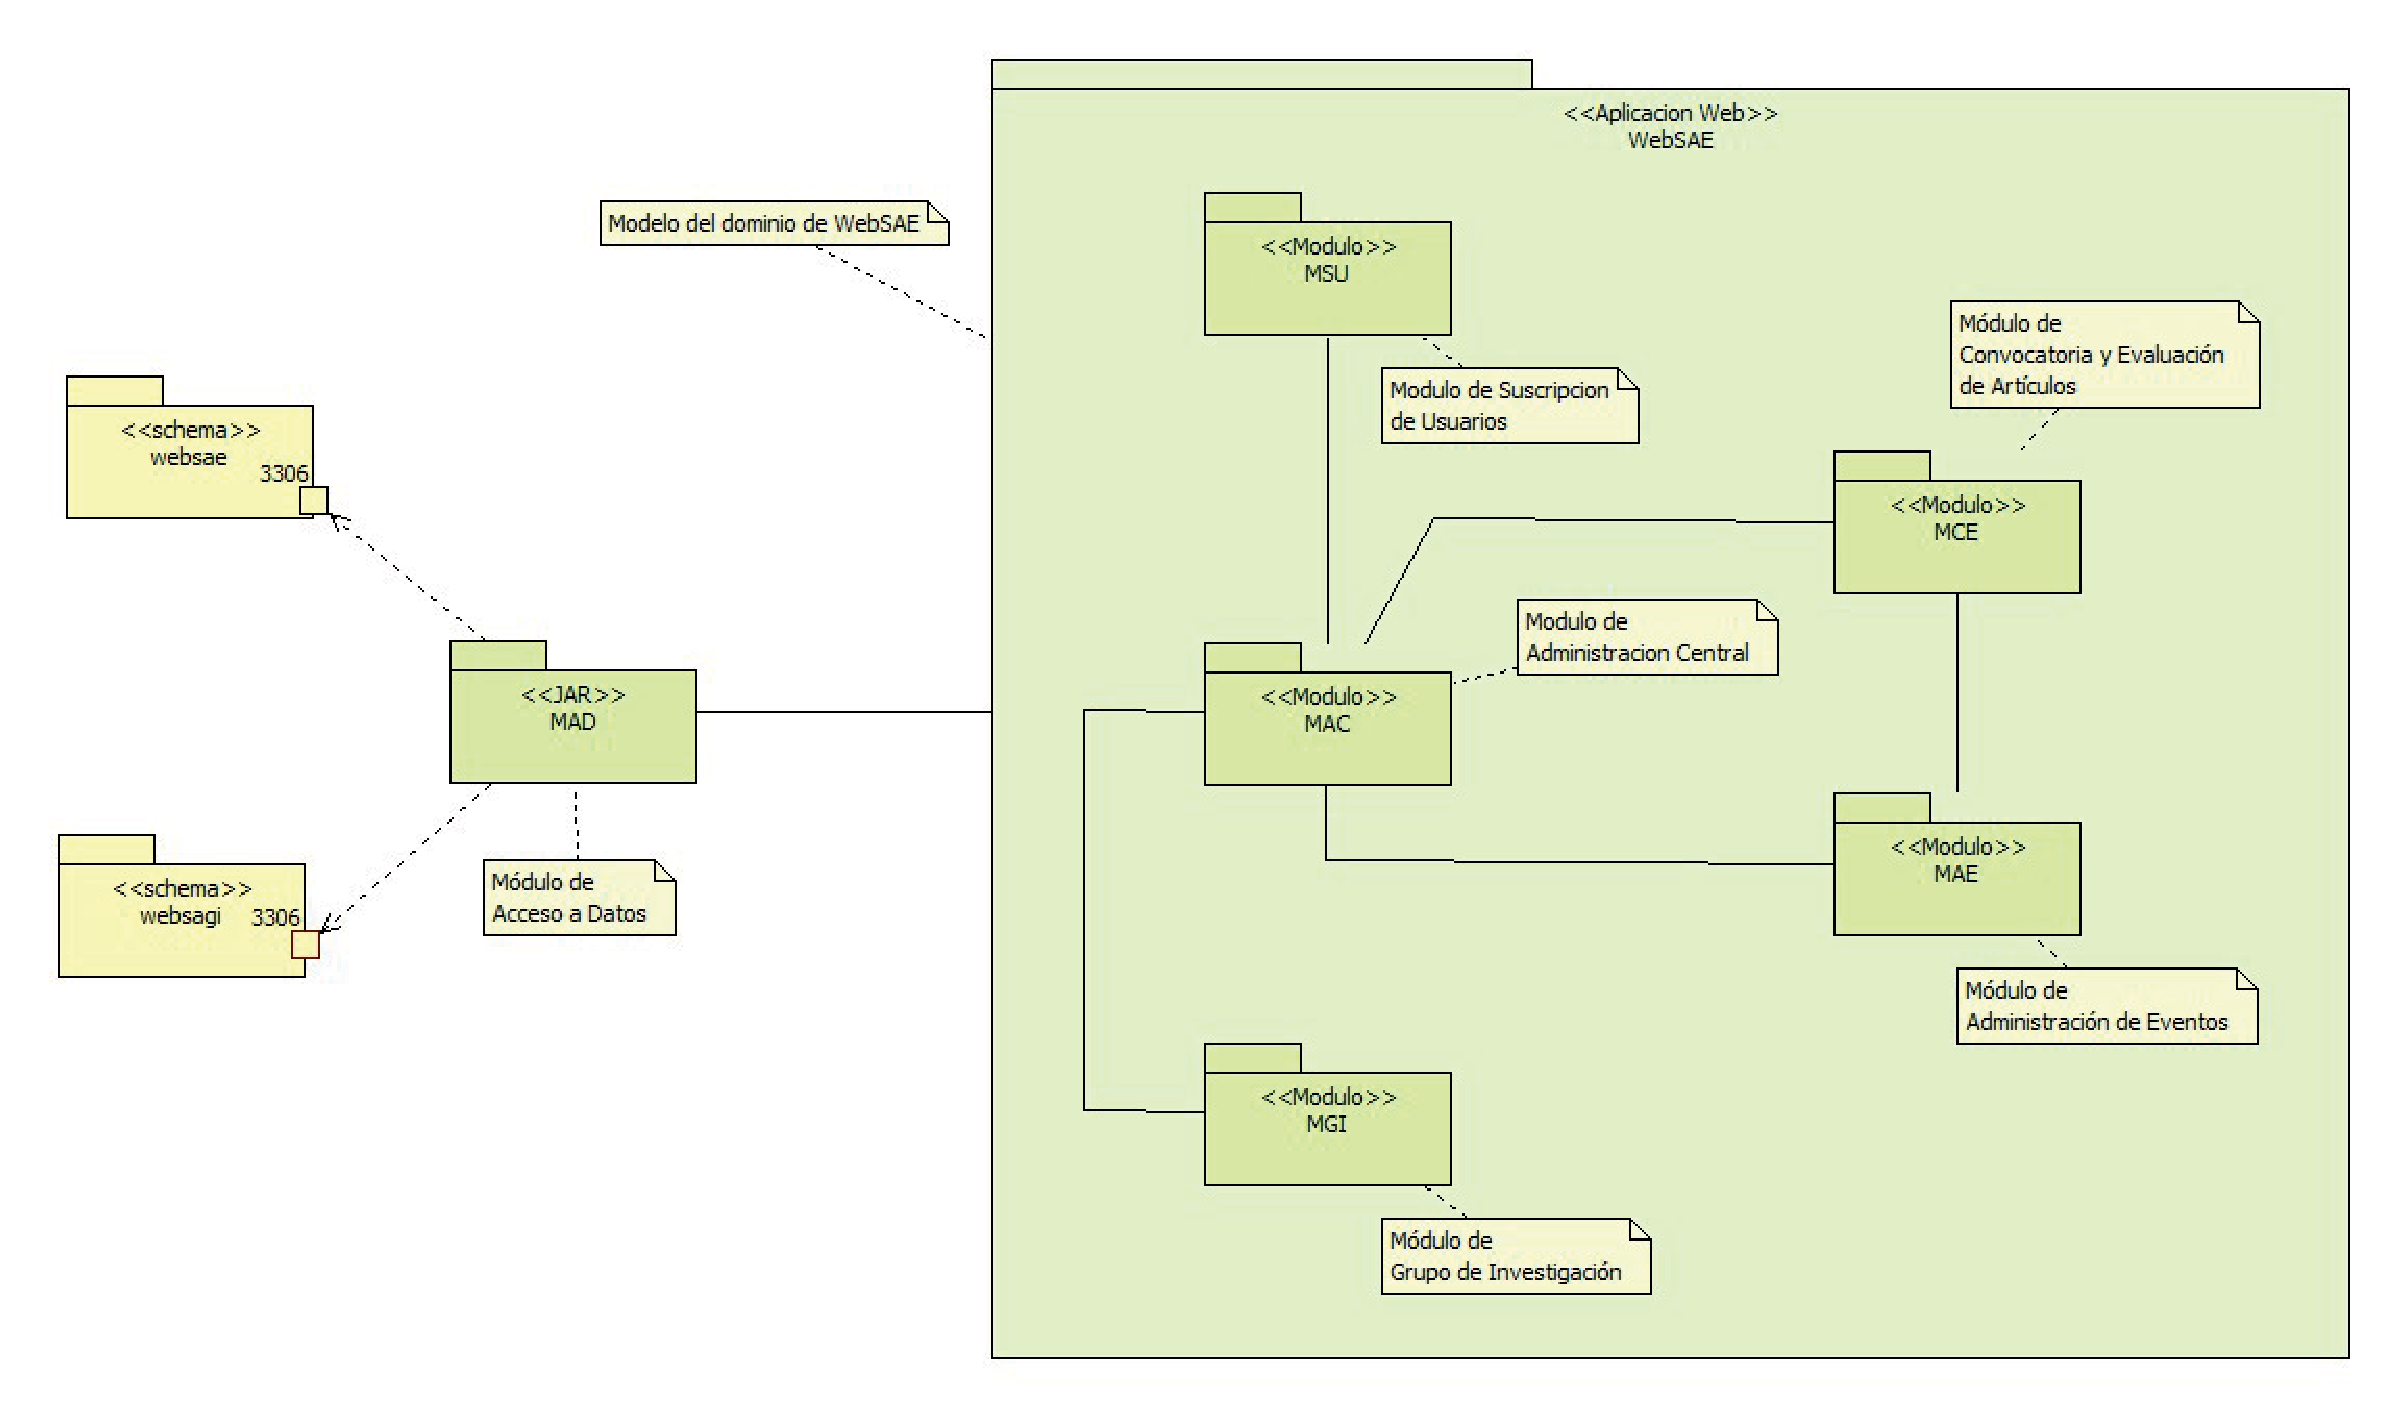
\includegraphics[width=1.4\textwidth]{images/websae-arquitectura.eps}}
  \caption{Dise\~no de la Arquitectura del Sistema de Administraci\'on de Eventos.}
  \label{websae:arquitectura}
\end{figure}
\end{landscape}

\end{indentar}

\subsection{M\'odulos del Sistema}
\begin{indentar}
\end{indentar}

\subsection{Arquitectura basada en patrones de dise\~no}
\begin{indentar}
\end{indentar}

\section{Diagrama de Clases del Sistema}
\begin{indentar}
\end{indentar}

\section{Modelo l\'ogico de la Base de Datos}
\begin{indentar}
\end{indentar}

\chapter{Implementaci\'on y Pruebas}
\begin{indentar}
\end{indentar}

\section{Capas del Sistema y comunicaci\'on entre capas}
\begin{indentar}
\end{indentar}

\subsection{Implementaci\'on basada en el an\'alisis con MERODE y MDA}
\begin{indentar}
\end{indentar}

\section{Plan de Pruebas}
\begin{indentar}
\end{indentar}

\section{Resultados de las Pruebas y M\'etricas tomadas}
\begin{indentar}
\end{indentar}

\chapter*{CONCLUSIONES Y RECOMENDACIONES}
\addcontentsline{toc}{chapter}{CONCLUSIONES}
\section{Comentarios generales}

\begin{indentar}
Luego de la elaboraci\'on del PSM de cada m\'odulo con su correspondiente PIM, se llev\'o a cabo la transformaci\'on deseada del c\'odigo, s\'olo del dise\~no del dominio.

En este punto es necesario comentar acerca de las herramientas que usamos para la generaci\'on deseada del PSM al c\'odigo, en primera instancia deseamos utilizar una herramienta llamada Magic Draw\footnote{\url{http://www.magicdraw.com/}}, una herramienta que no s\'olo nos gener\'o las clases propias del dominio, si no tambi\'en el correspondiente DDL\footnote{Data Definition Language} de la Base de Datos que nosotros hab\'iamos seleccionado; sin embargo, la curiosidad intelectual nos llev\'o a utilizar otra herramienta CASE Open Source para utilizar las metodolog\'ias MDA y MERODE en conjunto, y la que se seleccion\'o fue StarUML debido a sus singulares caracter\'isticas de las que en su momento deseamos aprovecharnos, pero existi\'o la gran desventaja que esta herramienta solo nos proporcion\'o la transformaci\'on del PSM al c\'odigo java.

La \'unica ventaja que se pudo sacar de esta herramienta fue la de conocer el hecho que se pueden implementar cartuchos para la transformaci\'on del PSM al c\'odigo, no s\'olo de la parte del dominio del sistema, si no tambi\'en de la capa controlador, que en el caso nuestro, fue implementado seg\'un la arquitectura J2EE.

Las ''transformaciones manuales'' que se realizaron en la mayor\'ia del proyecto, nos ayud\'o a la estandarizaci\'on del c\'odigo de la misma, conservando una gran similitud en la parte del c\'odigo en el lado del servidor y del cliente, conservando el patr\'on de dise\~no MVC 2 mencionado como requerimiento no funcional.
\end{indentar}

\include{anexos}

% This file is setup to use a bibtex file sample.bib and uses the
% plain style.  Note, the bibliography could come after the appendices.
\bibliographystyle{unsrt}
\bibliography{websae}


% Indices come here.

\end{document}
\endinput
%%
%% End of file `mitsample.tex'.
